\documentclass[aspectratio=169]{beamer}

\usepackage[T5]{fontenc}
\usepackage[utf8]{inputenc}
\usepackage{lmodern}

\usetheme{Madrid}

\usepackage{graphicx}
\usepackage{multicol}
\usepackage{amsmath,amssymb}

% Outline look: blue text, numbered, no balls
\setbeamertemplate{section in toc}{%
  \leavevmode\inserttocsectionnumber.~\inserttocsection\par}
\setbeamercolor{section in toc}{fg=blue}

\hypersetup{colorlinks=true, urlcolor=blue}

\newcommand{\backbtn}{%
  \hfill\hyperlink{outline}{\beamerbutton{Mục lục}}}


% Giảm khoảng cách trên/dưới công thức hiển thị để slide gọn hơn
\makeatletter
\def\tight@disp{\setlength\abovedisplayskip{4pt plus 2pt}%
  \setlength\belowdisplayskip{4pt plus 2pt}%
  \setlength\abovedisplayshortskip{2pt plus 1pt}%
  \setlength\belowdisplayshortskip{2pt plus 1pt}}
\g@addto@macro\normalsize{\tight@disp}
\g@addto@macro\small{\tight@disp}
\g@addto@macro\footnotesize{\tight@disp}
\g@addto@macro\scriptsize{\tight@disp}
\makeatother

\title[Ứng suất tiếp]{Ứng suất tiếp trong dầm và cấu kiện thành mỏng}
\author[© N. V. Sỹ]{Nguyễn Văn Sỹ}
\institute[TNUT]{%
  Bộ môn Hệ thống Công nghiệp \\
  Trường Đại học Kỹ thuật Công nghiệp \\
  \href{mailto:vansy@tnut.edu.vn}{vansy@tnut.edu.vn}}
\date[Cơ học vật liệu]{\large Cơ học vật liệu – Ứng suất tiếp trong dầm \\[0.5em] \footnotesize \copyright\ Nguyễn Văn Sỹ}

\begin{document}

\begin{frame}
  \titlepage
\end{frame}
%====================
\begin{frame}{Tài liệu tham khảo}
	\small
	F. P. Beer, E. R. Johnston, Jr., J. T. DeWolf, D. F. Mazurek,
	\emph{Mechanics of Materials}, 6th ed., McGraw-Hill, New York, 2012.
	
	\vspace{1em}
	\footnotesize\color{gray}
	Toàn bộ hình vẽ trong bài giảng được trích từ giáo trình trên, chỉ sử dụng
	cho mục đích giảng dạy nội bộ.
\end{frame}
% ===== OUTLINE SLIDE =====
\begin{frame}[t]{Nội dung}
  \hypertarget{outline}{}
  \tiny
  \begin{multicols}{2}
    \tableofcontents[hideallsubsections]
  \end{multicols}
\end{frame}

% ===== CONTENT SLIDES =====
\section{Giới thiệu}
\begin{frame}[t]{Giới thiệu}
  \begin{columns}[T]
    \column{0.60\textwidth}
      \small
      \begin{itemize}
        \setlength{\itemsep}{0.4em}
        \item Tải trọng ngang tác dụng lên dầm gây ra ứng suất pháp và ứng
              suất tiếp trên các mặt cắt ngang.
        \item Phân bố ứng suất pháp và ứng suất tiếp thỏa mãn:
        \[
          \begin{aligned}
            F_x &= \int\sigma_x\,dA = 0 & M_x &= \int(y\tau_{xz} - z\tau_{xy})\,dA = 0\\
            F_y &= \int\tau_{xy}\,dA = -V & M_y &= \int z\sigma_x\,dA = 0\\
            F_z &= \int\tau_{xz}\,dA = 0 & M_z &= \int(-y\sigma_x)\,dA = M
          \end{aligned}
        \]
        \item Khi có ứng suất tiếp tác dụng trên các mặt đứng của một phân
              tố, phải có các ứng suất bằng như vậy tác dụng trên các mặt
              nằm ngang.
        \item Ứng suất tiếp dọc phải tồn tại trong mọi cấu kiện chịu tải
              trọng ngang.
      \end{itemize}
    \column{0.38\textwidth}
      \centering
      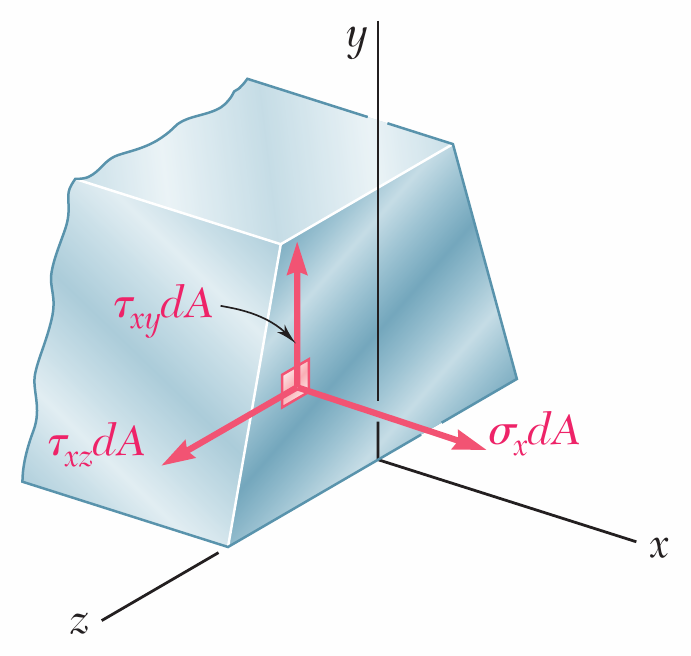
\includegraphics[width=\linewidth,height=2.9cm,keepaspectratio]{Chap_6/fig_6_1.png}\\[2pt]
      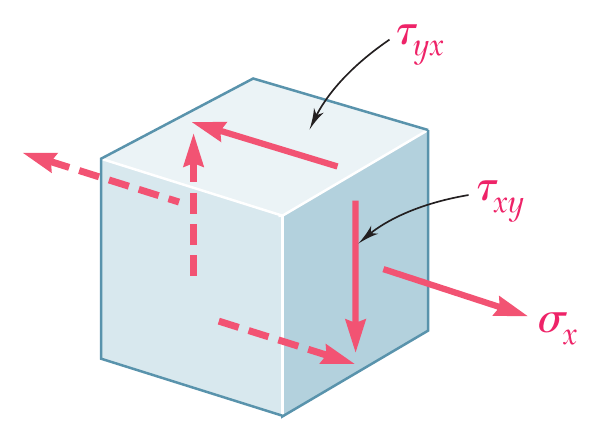
\includegraphics[width=\linewidth,height=2.9cm,keepaspectratio]{Chap_6/fig_6_2.png}
  \end{columns}
\end{frame}
% ===========
\section{Lực cắt trên mặt nằm ngang của phân tố dầm}
\begin{frame}[t]{Lực cắt trên mặt nằm ngang của phân tố dầm}
  \begin{columns}[T]
    \column{0.60\textwidth}
      \small
      \begin{itemize}
        \setlength{\itemsep}{0.4em}
        \item Xét dầm lăng trụ.
        \item Cân bằng của phân tố dầm:
        \[
          \textstyle\sum F_x = 0 = \Delta H + \int_A(\sigma_D - \sigma_C)\,dA
        \]
        \[
          \Delta H = \frac{M_D - M_C}{I}\int_A y\,dA
        \]
        \item Lưu ý:
        \[
          Q = \int_A y\,dA \qquad
          M_D - M_C = \frac{dM}{dx}\Delta x = V\Delta x
        \]
        \item Thay vào:
        \[
          \Delta H = \frac{VQ}{I}\Delta x
          \qquad
          q = \frac{\Delta H}{\Delta x} = \frac{VQ}{I} = \text{dòng lực cắt}
        \]
      \end{itemize}
    \column{0.38\textwidth}
      \centering
      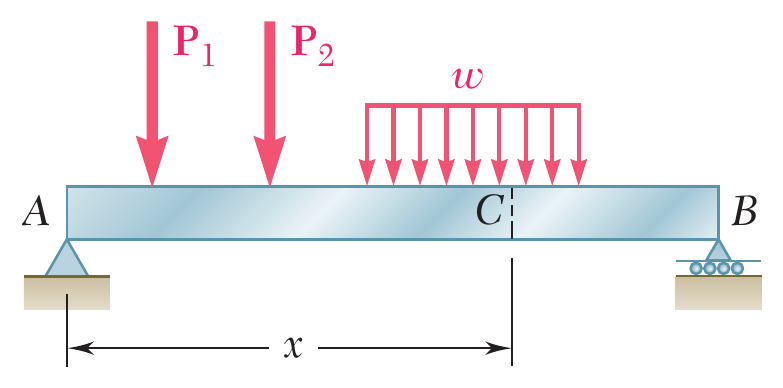
\includegraphics[width=\linewidth,height=1.9cm,keepaspectratio]{Chap_6/fig_6_4_a.png}\\[2pt]
      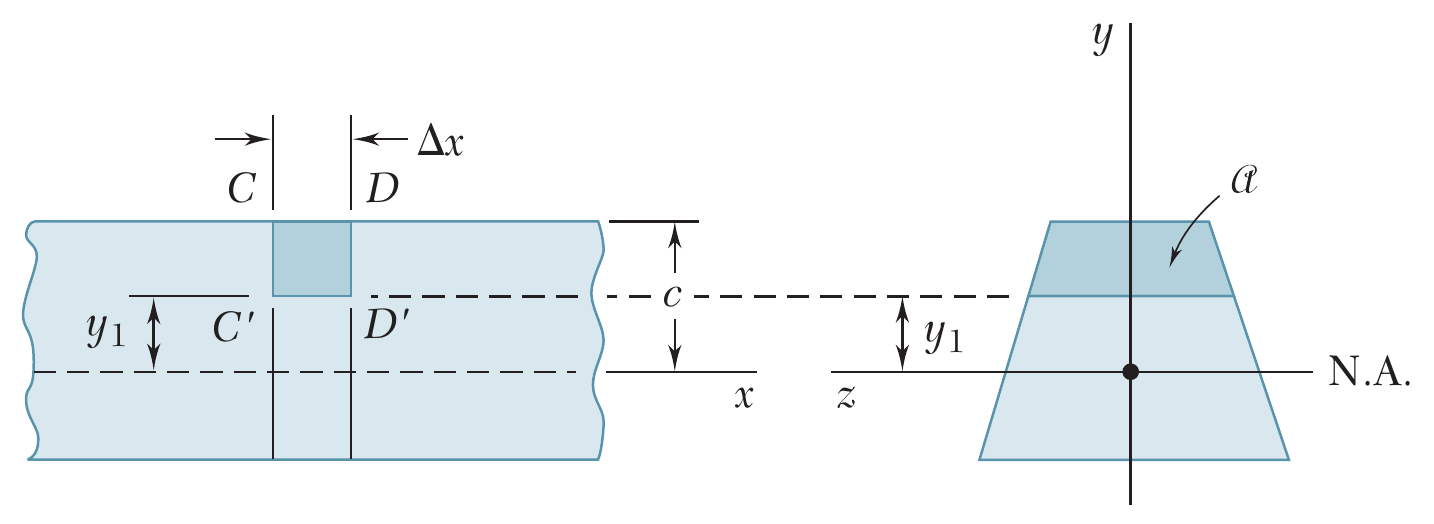
\includegraphics[width=\linewidth,height=1.9cm,keepaspectratio]{Chap_6/fig_6_5.png}\\[2pt]
      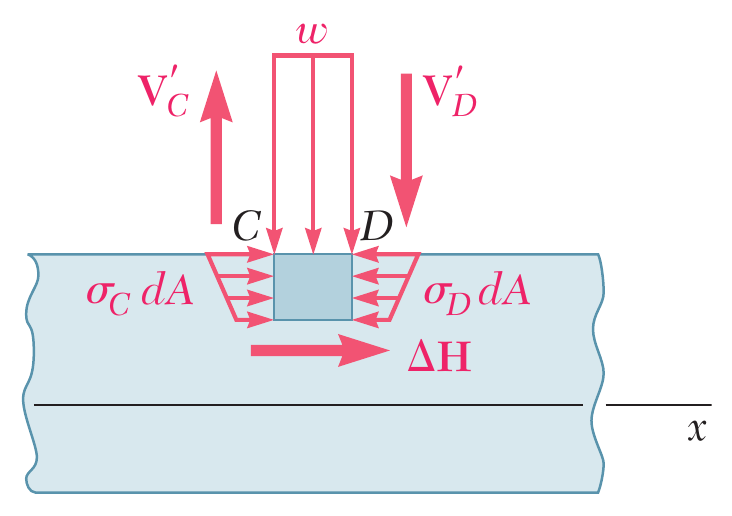
\includegraphics[width=\linewidth,height=1.9cm,keepaspectratio]{Chap_6/fig_6_6.png}
  \end{columns}
\end{frame}
% ===========
\begin{frame}[t]{Lực cắt trên mặt nằm ngang của phân tố dầm (tiếp)}
  \begin{columns}[T]
    \column{0.60\textwidth}
      \footnotesize
      \begin{itemize}
        \setlength{\itemsep}{0.25em}
        \item Dòng lực cắt:
        \[
          q = \frac{\Delta H}{\Delta x} = \frac{VQ}{I} = \text{dòng lực cắt}
        \]
        \item trong đó
        \[
          Q = \int_A y\,dA
        \]
        = mô men tĩnh của phần diện tích phía trên $y_1$
        \[
          I = \int_{A+A'} y^2\,dA
        \]
        = mô men quán tính của toàn bộ mặt cắt
        \item Kết quả tương tự cho phần diện tích phía dưới:
        \[
          q' = \frac{\Delta H'}{\Delta x} = \frac{VQ'}{I} = -q
        \]
        \[
          Q + Q' = 0 \qquad \Delta H' = -\Delta H
        \]
        ($Q + Q'$ = mô men tĩnh đối với trục trung hòa)
      \end{itemize}
    \column{0.38\textwidth}
      \centering
      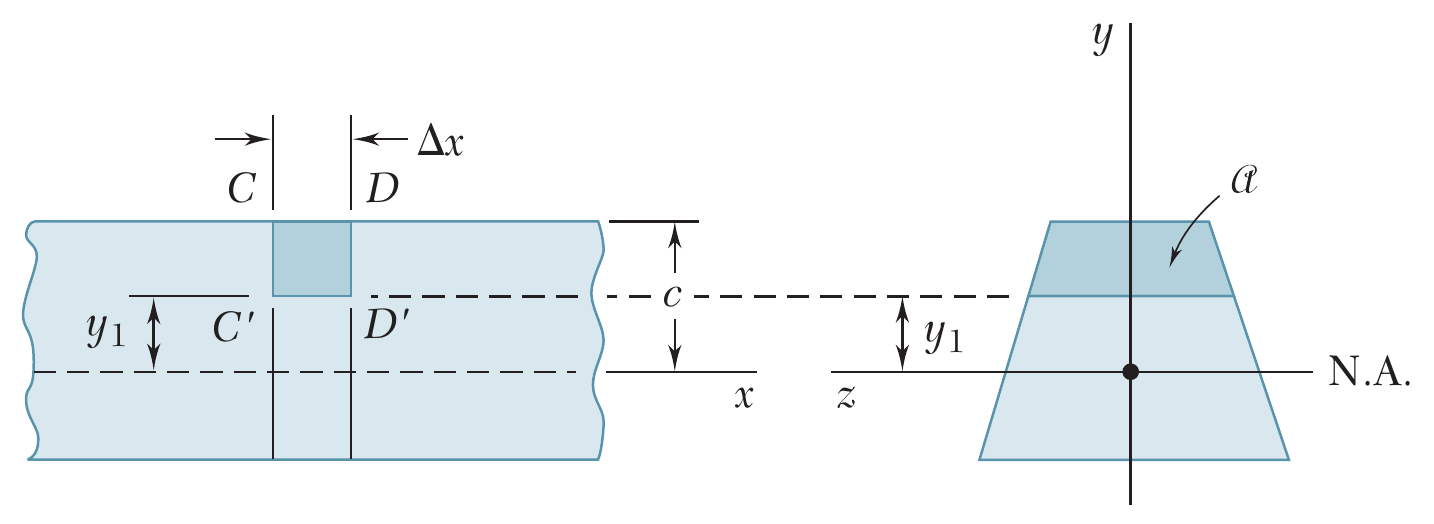
\includegraphics[width=\linewidth,height=2.5cm,keepaspectratio]{Chap_6/fig_6_5.png}\\[2pt]
      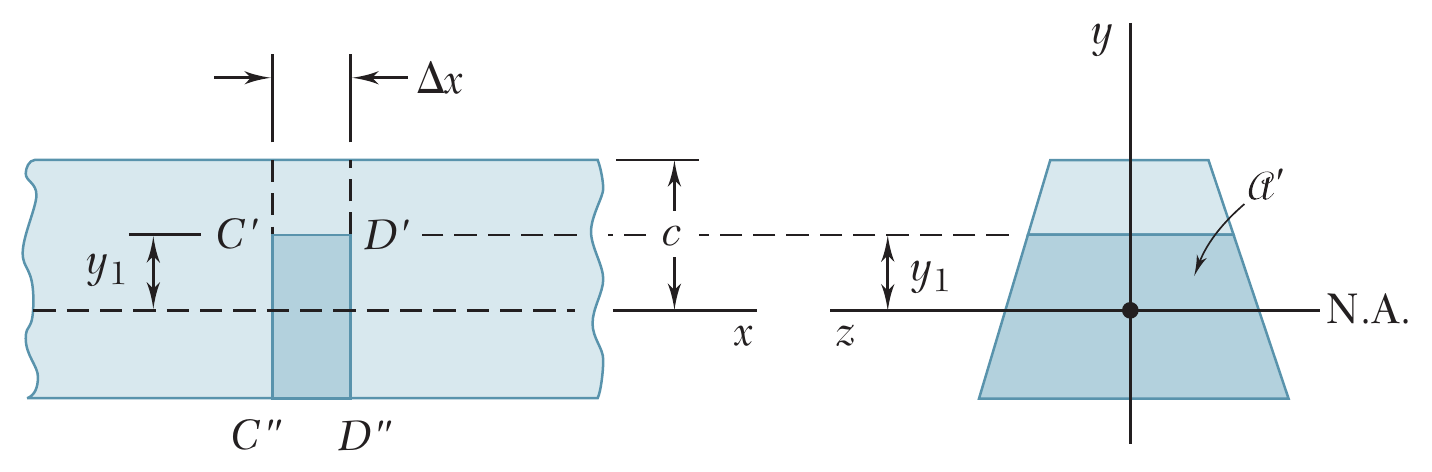
\includegraphics[width=\linewidth,height=2.5cm,keepaspectratio]{Chap_6/fig_6_7.png}
  \end{columns}
\end{frame}
% ===========
\section{Ví dụ 6.01}
\begin{frame}[t]{Ví dụ 6.01}
  \begin{columns}[T]
    \column{0.42\textwidth}
      \centering
      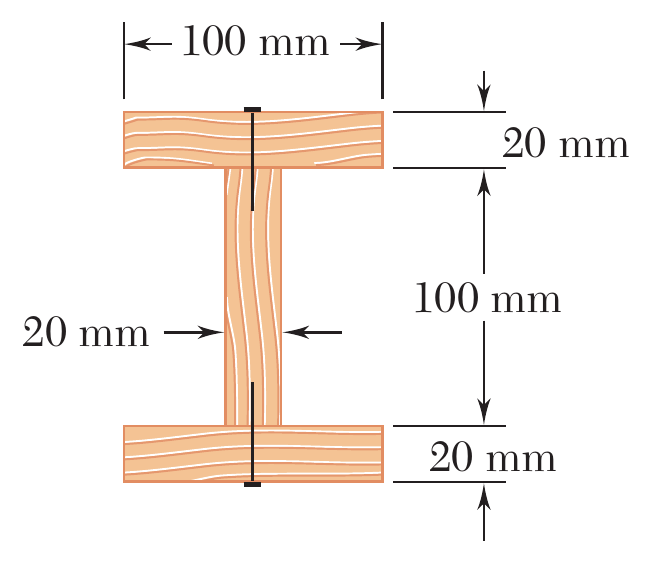
\includegraphics[width=\linewidth,height=5.5cm,keepaspectratio]{Chap_6/fig_6_8.png}
    \column{0.56\textwidth}
      \small
      Một dầm được làm từ ba tấm ván đóng đinh với nhau. Biết khoảng cách
      giữa các đinh là 25 mm và lực cắt đứng trong dầm là $V = 500\,\mathrm{N}$,
      xác định lực cắt tác dụng lên mỗi đinh.

      \vspace{0.8em}
      \textbf{LỜI GIẢI:}
      \begin{itemize}
        \setlength{\itemsep}{0.5em}
        \item Xác định lực ngang trên một đơn vị chiều dài, hay dòng lực cắt
              $q$, trên mặt dưới của tấm ván trên.
        \item Tính lực cắt tương ứng trong mỗi đinh.
      \end{itemize}
  \end{columns}
\end{frame}
% ===========
\begin{frame}[t]{Ví dụ 6.01 (tiếp)}
  \begin{columns}[T]
    \column{0.60\textwidth}
      \small
      \textbf{LỜI GIẢI:}
      \begin{itemize}
        \setlength{\itemsep}{0.4em}
        \item Xác định lực ngang trên một đơn vị chiều dài, hay dòng lực cắt
              $q$, trên mặt dưới của tấm ván trên:
        \[
          Q = A\bar{y} = (0{,}020\times0{,}100)(0{,}060) = 120\times10^{-6}\,\mathrm{m}^3
        \]
        \[
          I = \tfrac{1}{12}(0{,}020)(0{,}100)^3
        \]
        \[
          \quad + 2\left[\tfrac{1}{12}(0{,}100)(0{,}020)^3 + (0{,}020\times0{,}100)(0{,}060)^2\right]
        \]
        \[
          I = 16{,}20\times10^{-6}\,\mathrm{m}^4
        \]
        \[
          q = \frac{VQ}{I} = \frac{(500\,\mathrm{N})(120\times10^{-6}\,\mathrm{m}^3)}{16{,}20\times10^{-6}\,\mathrm{m}^4}
            = 3704\,\mathrm{N/m}
        \]
        \item Tính lực cắt tương ứng trong mỗi đinh với bước đinh 25 mm:
        \[
          F = (0{,}025)q = (0{,}025)(3704)
          \qquad \boxed{F = 92{,}6\,\mathrm{N}}
        \]
      \end{itemize}
    \column{0.38\textwidth}
      \centering
      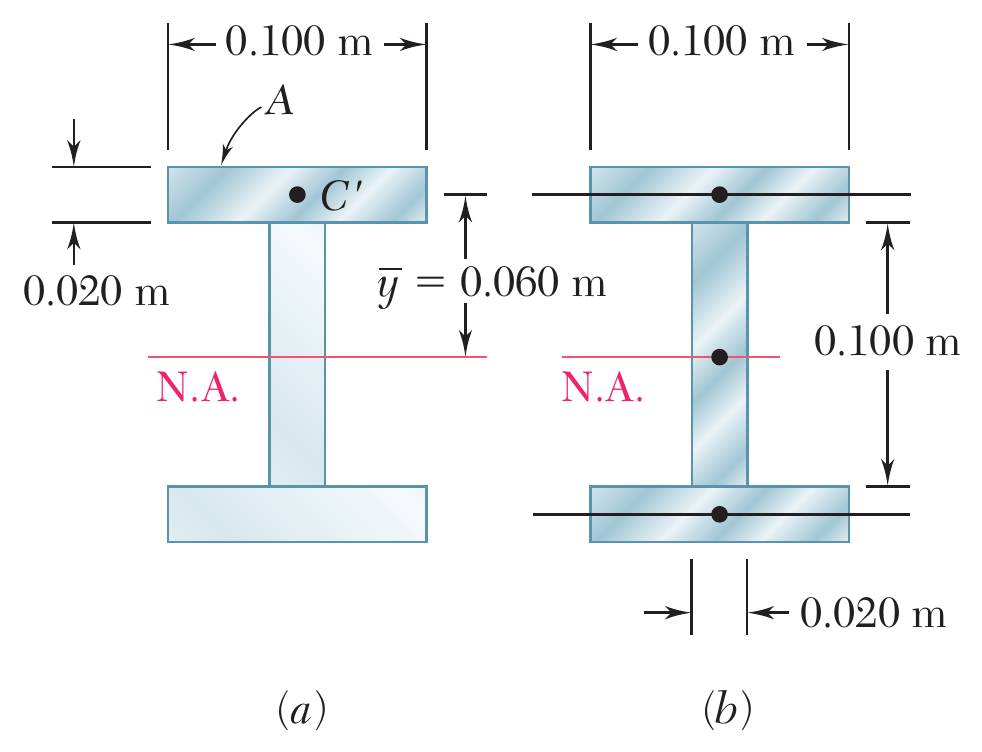
\includegraphics[width=\linewidth,height=5.5cm,keepaspectratio]{Chap_6/fig_6_9.png}
  \end{columns}
\end{frame}
% ===========
\section{Xác định ứng suất tiếp trong dầm}
\begin{frame}[t]{Xác định ứng suất tiếp trong dầm}
  \begin{columns}[T]
    \column{0.58\textwidth}
      \small
      \begin{itemize}
        \setlength{\itemsep}{0.6em}
        \item Ứng suất tiếp trung bình trên mặt nằm ngang của phân tố bằng
              lực cắt trên phân tố chia cho diện tích mặt đó:
        \[
          \tau_{\mathrm{tb}} = \frac{\Delta H}{\Delta A} = \frac{q\Delta x}{\Delta A}
            = \frac{VQ}{I}\frac{\Delta x}{t\Delta x} = \frac{VQ}{It}
        \]
        \item Trên mặt trên và mặt dưới của dầm, $\tau_{yx} = 0$. Suy ra
              $\tau_{xy} = 0$ tại mép trên và mép dưới của mặt cắt ngang.
        \item Nếu bề rộng dầm tương đương hoặc lớn so với chiều cao, ứng suất
              tiếp tại $D_1$ và $D_2$ lớn hơn đáng kể so với tại $D$.
      \end{itemize}
    \column{0.40\textwidth}
      \centering
      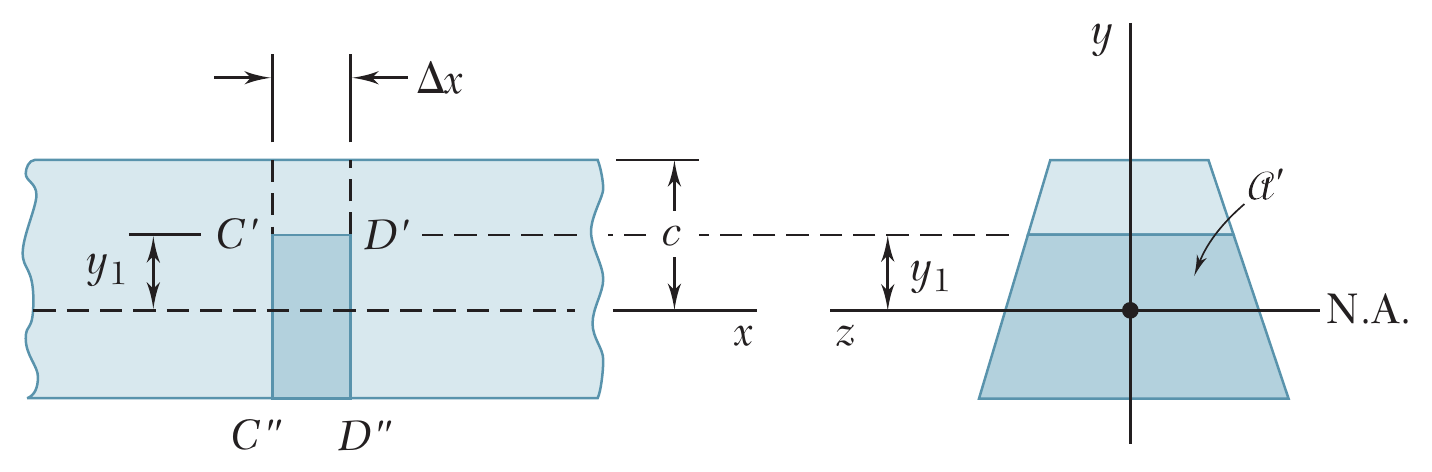
\includegraphics[width=\linewidth,height=1.9cm,keepaspectratio]{Chap_6/fig_6_7.png}\\[2pt]
      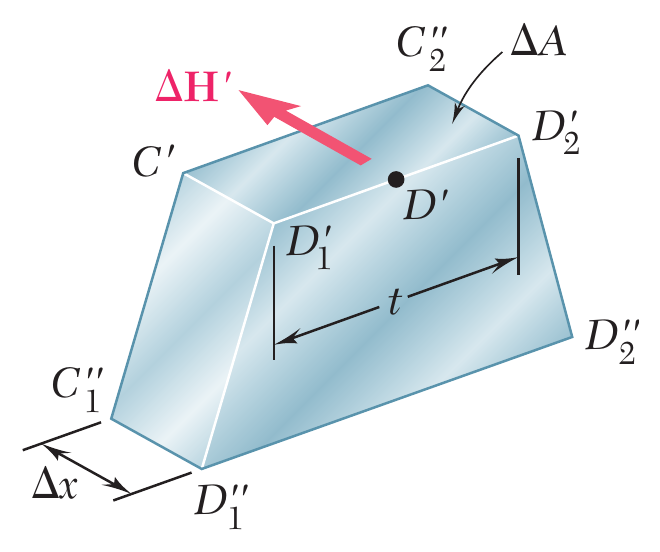
\includegraphics[width=\linewidth,height=1.9cm,keepaspectratio]{Chap_6/fig_6_10.png}\\[2pt]
      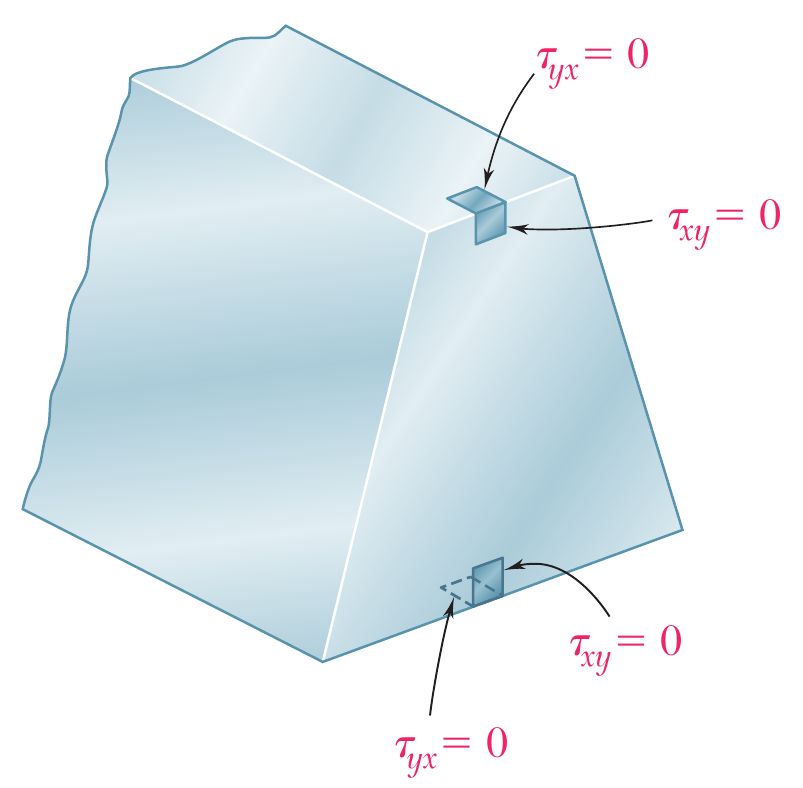
\includegraphics[width=\linewidth,height=1.9cm,keepaspectratio]{Chap_6/fig_6_12.png}
  \end{columns}
\end{frame}
% ===========
\section{Ứng suất tiếp trong các loại dầm thông dụng}
\begin{frame}[t]{Ứng suất tiếp $\tau_{xy}$ trong các loại dầm thông dụng}
  \begin{columns}[T]
    \column{0.58\textwidth}
      \small
      \begin{itemize}
        \setlength{\itemsep}{0.6em}
        \item Với dầm chữ nhật hẹp:
        \[
          \tau_{xy} = \frac{VQ}{Ib} = \frac{3}{2}\frac{V}{A}\left(1 - \frac{y^2}{c^2}\right)
        \]
        \[
          \tau_{\max} = \frac{3}{2}\frac{V}{A}
        \]
        \item Với dầm tiêu chuẩn Mỹ (dầm S) và dầm cánh rộng (dầm W):
        \[
          \tau_{\mathrm{tb}} = \frac{VQ}{It}
          \qquad
          \tau_{\max} = \frac{V}{A_{\text{bụng}}}
        \]
      \end{itemize}
    \column{0.40\textwidth}
      \centering
      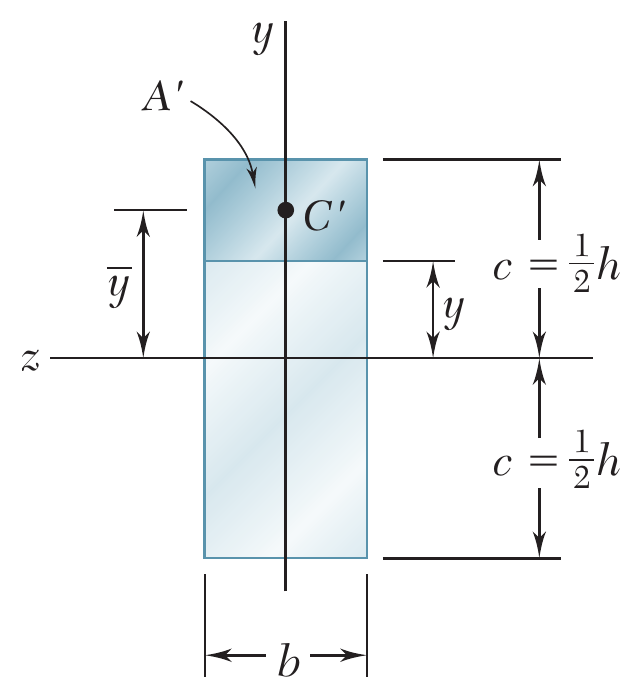
\includegraphics[width=\linewidth,height=2.9cm,keepaspectratio]{Chap_6/fig_6_14.png}\\[2pt]
      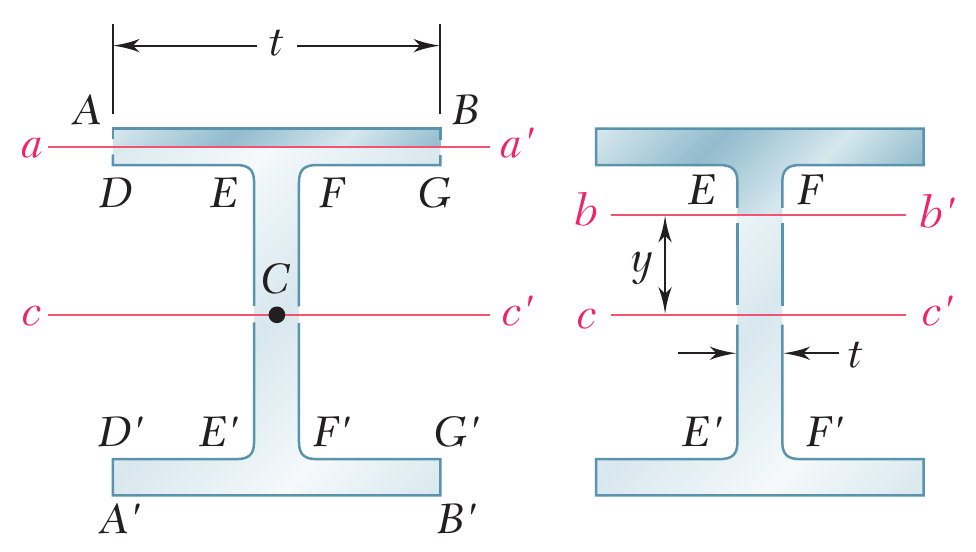
\includegraphics[width=\linewidth,height=2.9cm,keepaspectratio]{Chap_6/fig_6_16.png}
  \end{columns}
\end{frame}
% ===========
\section{Phân bố ứng suất trong dầm chữ nhật hẹp}
\begin{frame}[t]{Thảo luận thêm về phân bố ứng suất trong dầm chữ nhật hẹp}
  \begin{columns}[T]
    \column{0.58\textwidth}
      \small
      \begin{itemize}
        \setlength{\itemsep}{0.4em}
        \item Xét dầm công xôn chữ nhật hẹp chịu lực $P$ ở đầu tự do:
        \[
          \tau_{xy} = \frac{3}{2}\frac{P}{A}\left(1 - \frac{y^2}{c^2}\right)
          \qquad
          \sigma_x = +\frac{Pxy}{I}
        \]
        \item Ứng suất tiếp không phụ thuộc vào khoảng cách đến điểm đặt
              lực.
        \item Biến dạng dài và ứng suất pháp không bị ảnh hưởng bởi ứng suất
              tiếp.
        \item Theo nguyên lý Saint-Venant, ảnh hưởng của cách đặt tải là
              không đáng kể, trừ vùng lân cận ngay sát điểm đặt lực.
        \item Sai lệch ứng suất/biến dạng đối với tải trọng phân bố là không
              đáng kể với các mặt cắt dầm thông thường.
      \end{itemize}
    \column{0.40\textwidth}
      \centering
      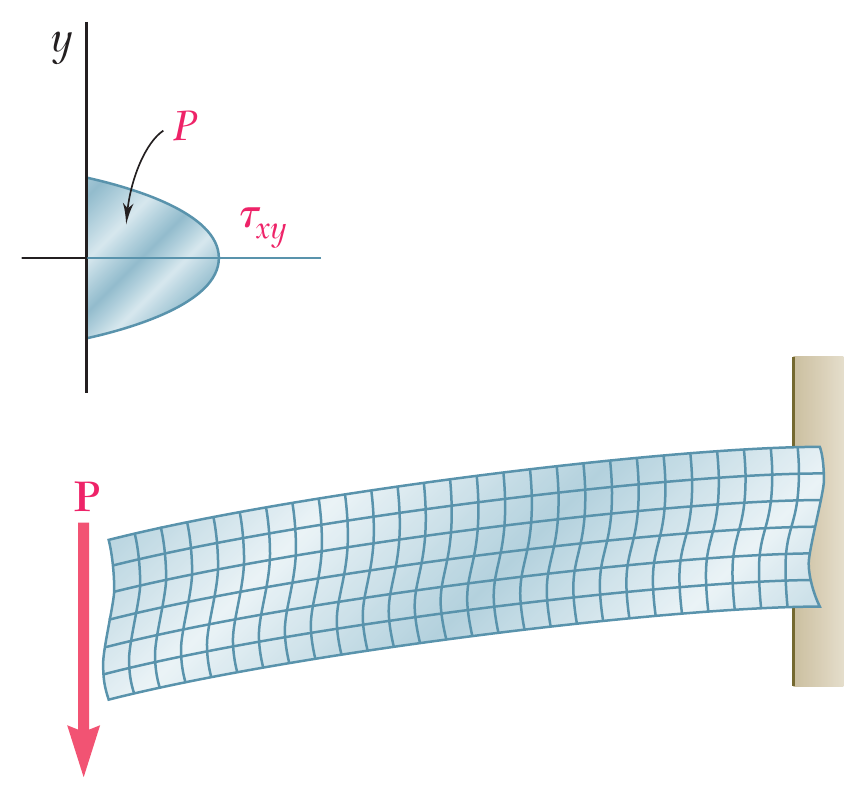
\includegraphics[width=\linewidth,height=1.9cm,keepaspectratio]{Chap_6/fig_6_19.png}\\[2pt]
      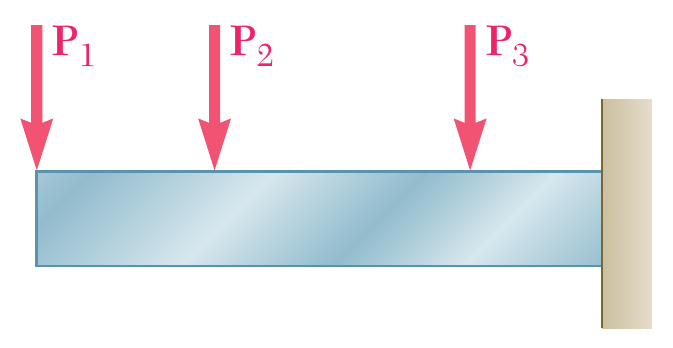
\includegraphics[width=\linewidth,height=1.9cm,keepaspectratio]{Chap_6/fig_6_20.png}\\[2pt]
      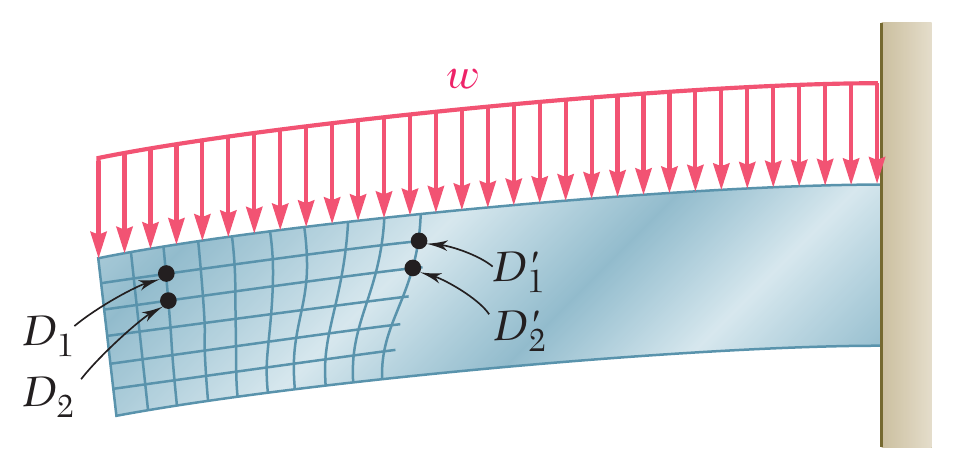
\includegraphics[width=\linewidth,height=1.9cm,keepaspectratio]{Chap_6/fig_6_21.png}
  \end{columns}
\end{frame}
% ===========
\section{Bài mẫu 6.2}
\begin{frame}[t]{Bài mẫu 6.2}
  \begin{columns}[T]
    \column{0.42\textwidth}
      \centering
      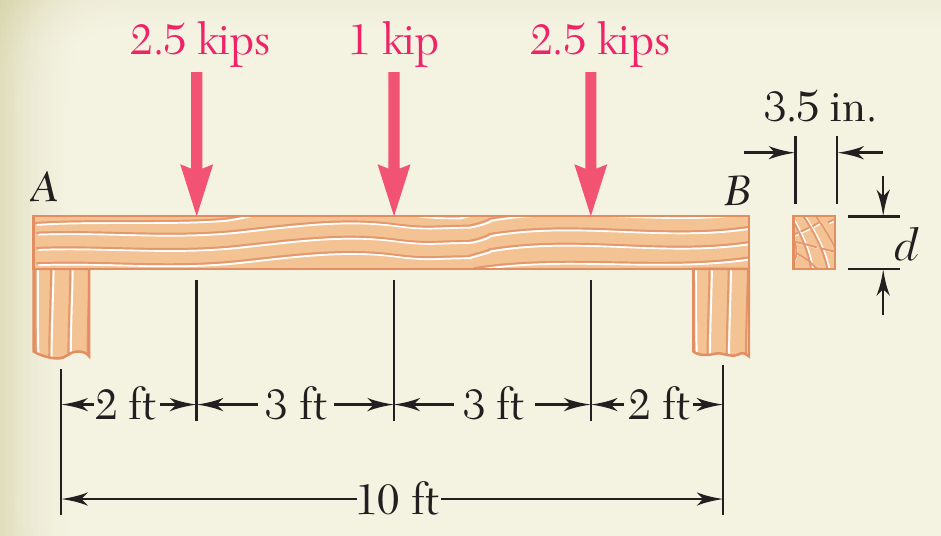
\includegraphics[width=\linewidth,height=5.5cm,keepaspectratio]{Chap_6/sp_6_2_a.png}
    \column{0.56\textwidth}
      \small
      Một dầm gỗ chịu ba tải trọng tập trung như hình vẽ. Biết rằng với
      loại gỗ sử dụng:
      \[
        \sigma_{\mathrm{all}} = 12\,\mathrm{MPa} \qquad
        \tau_{\mathrm{all}} = 0{,}8\,\mathrm{MPa}
      \]
      xác định chiều cao $d$ nhỏ nhất cần thiết của dầm.

      \vspace{0.3em}
      \textbf{LỜI GIẢI:}
      \begin{itemize}
        \setlength{\itemsep}{0.3em}
        \item Vẽ biểu đồ lực cắt và mô men uốn. Xác định các giá trị lớn nhất.
        \item Xác định chiều cao dầm theo ứng suất pháp cho phép.
        \item Xác định chiều cao dầm theo ứng suất tiếp cho phép.
        \item Chiều cao dầm cần thiết bằng giá trị lớn hơn trong hai chiều
              cao tìm được.
      \end{itemize}
  \end{columns}
\end{frame}
% ===========
\begin{frame}[t]{Bài mẫu 6.2 (tiếp)}
  \begin{columns}[T]
    \column{0.36\textwidth}
      \small
      \textbf{LỜI GIẢI:}

      \vspace{0.5em}
      Vẽ biểu đồ lực cắt và mô men uốn. Xác định các giá trị lớn nhất:
      \[
        |V|_{\max} = 14{,}5\,\mathrm{kN}
      \]
      \[
        |M|_{\max} = 10{,}95\,\mathrm{kN\cdot m}
      \]
    \column{0.62\textwidth}
      \centering
      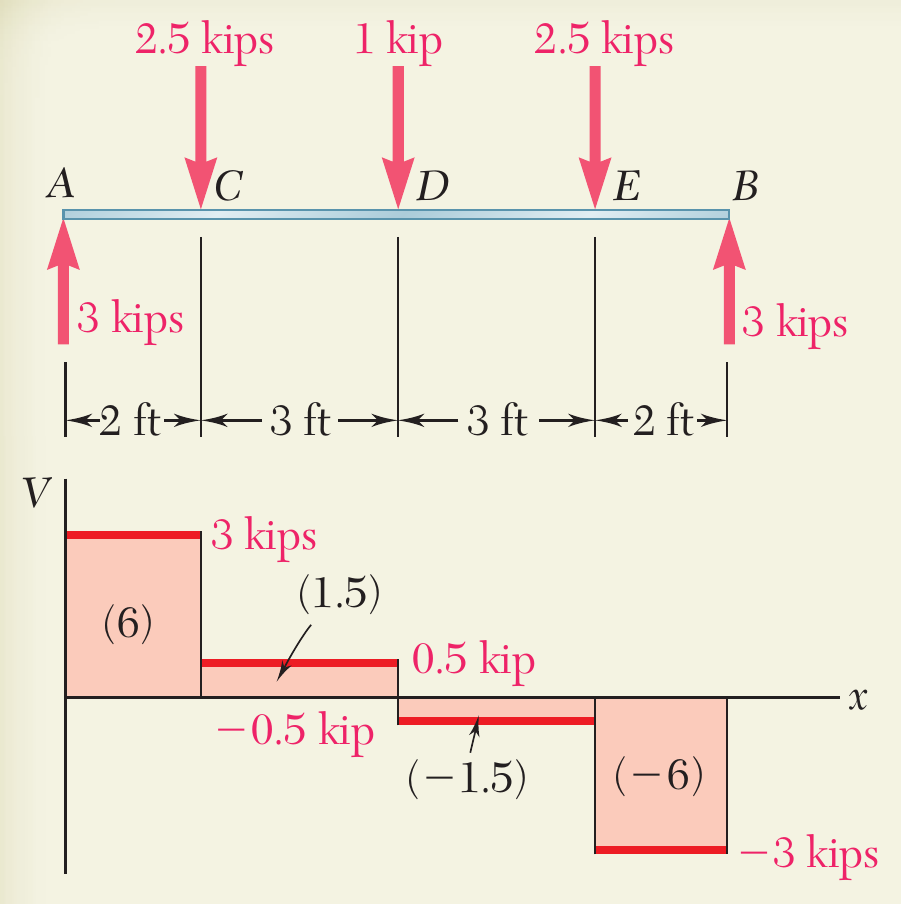
\includegraphics[width=\linewidth,height=6cm,keepaspectratio]{Chap_6/sp_6_2_b.png}
  \end{columns}
\end{frame}
% ===========
\begin{frame}[t]{Bài mẫu 6.2 (tiếp)}
  \begin{columns}[T]
    \column{0.60\textwidth}
      \small
      \[
        I = \tfrac{1}{12}bd^3 \qquad
        S = \frac{I}{c} = \tfrac{1}{6}bd^2 = \tfrac{1}{6}(0{,}09\,\mathrm{m})d^2
          = (0{,}015\,\mathrm{m})d^2
      \]
      \begin{itemize}
        \setlength{\itemsep}{0.5em}
        \item Xác định chiều cao dầm theo ứng suất pháp cho phép:
        \[
          \sigma_{\mathrm{all}} = \frac{|M|_{\max}}{S}
          \qquad
          12\times10^{6}\,\mathrm{Pa} = \frac{10{,}95\times10^{3}\,\mathrm{N\cdot m}}{(0{,}015\,\mathrm{m})d^2}
        \]
        \[
          d = 0{,}246\,\mathrm{m} = 246\,\mathrm{mm}
        \]
        \item Xác định chiều cao dầm theo ứng suất tiếp cho phép:
        \[
          \tau_{\mathrm{all}} = \frac{3}{2}\frac{|V|_{\max}}{A}
          \qquad
          0{,}8\times10^{6}\,\mathrm{Pa} = \frac{3}{2}\frac{14500\,\mathrm{N}}{(0{,}09\,\mathrm{m})d}
        \]
        \[
          d = 0{,}322\,\mathrm{m} = 322\,\mathrm{mm}
        \]
        \item Chiều cao dầm cần thiết bằng giá trị lớn hơn:
              \quad $\boxed{d = 322\,\mathrm{mm}}$
      \end{itemize}
    \column{0.38\textwidth}
      \centering
      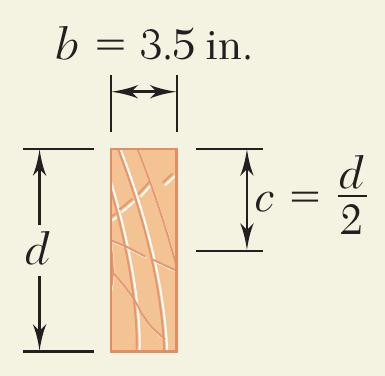
\includegraphics[width=\linewidth,height=5.5cm,keepaspectratio]{Chap_6/sp_6_2_c.png}
  \end{columns}
\end{frame}
% ===========
\section{Lực cắt dọc trên phân tố dầm có hình dạng bất kỳ}
\begin{frame}[t]{Lực cắt dọc trên phân tố dầm có hình dạng bất kỳ}
  \begin{columns}[T]
    \column{0.58\textwidth}
      \small
      \begin{itemize}
        \setlength{\itemsep}{0.6em}
        \item Ta đã xét phân bố của thành phần thẳng đứng $\tau_{xy}$ trên
              mặt cắt ngang của dầm. Bây giờ ta xét thành phần nằm ngang
              $\tau_{xz}$ của ứng suất.
        \item Xét dầm lăng trụ với một phân tố được xác định bởi mặt cong
              $CDD'C'$:
        \[
          \textstyle\sum F_x = 0 = \Delta H + \int_a(\sigma_D - \sigma_C)\,dA
        \]
        \item Ngoại trừ sự khác biệt về miền tích phân, kết quả này giống kết
              quả đã nhận được trước đây, dẫn tới:
        \[
          \Delta H = \frac{VQ}{I}\Delta x
          \qquad
          q = \frac{\Delta H}{\Delta x} = \frac{VQ}{I}
        \]
      \end{itemize}
    \column{0.40\textwidth}
      \centering
      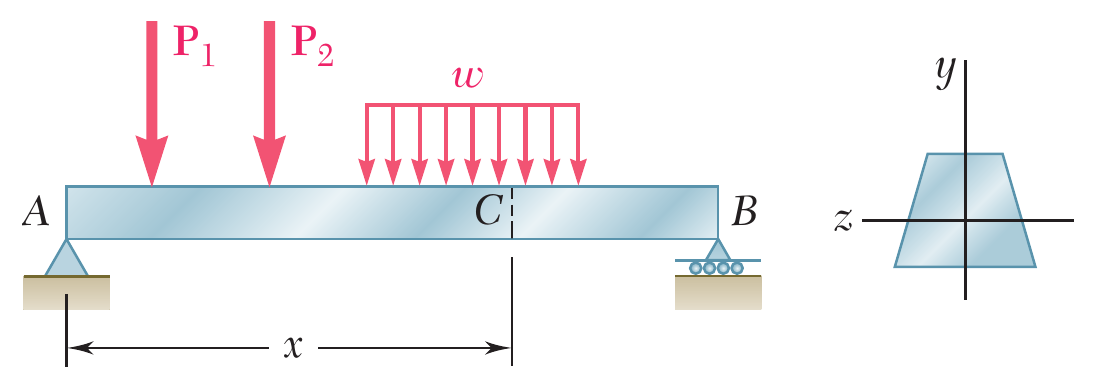
\includegraphics[width=\linewidth,height=1.9cm,keepaspectratio]{Chap_6/fig_6_4_b.png}\\[2pt]
      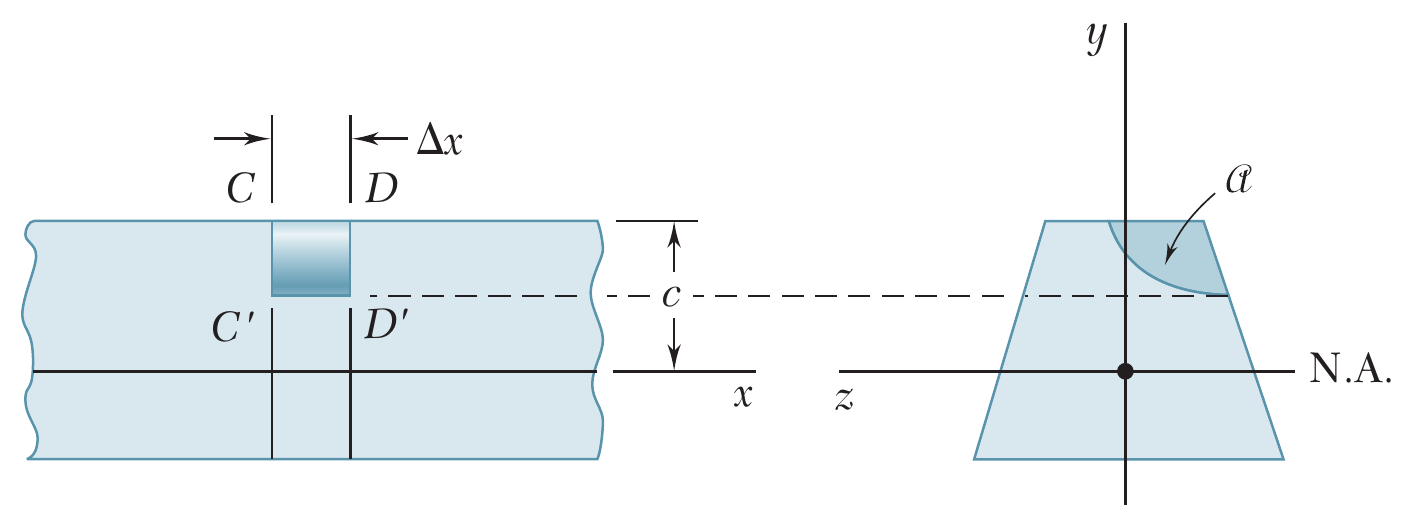
\includegraphics[width=\linewidth,height=1.9cm,keepaspectratio]{Chap_6/fig_6_23.png}\\[2pt]
      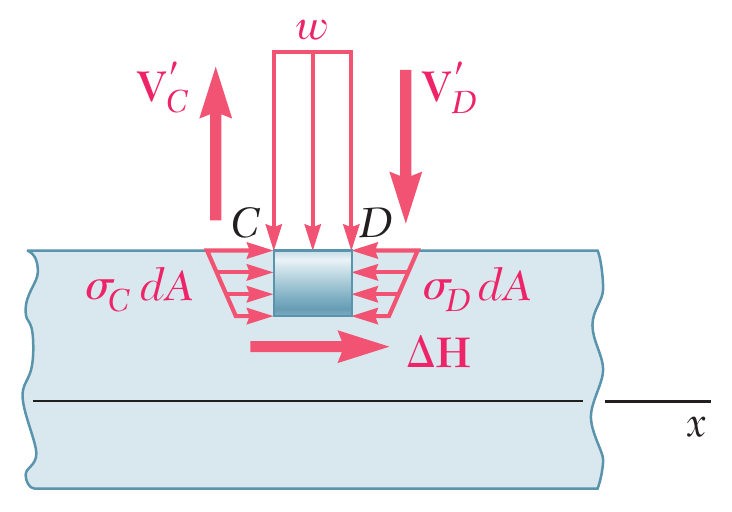
\includegraphics[width=\linewidth,height=1.9cm,keepaspectratio]{Chap_6/fig_6_24.png}
  \end{columns}
\end{frame}
% ===========
\section{Ví dụ 6.04}
\begin{frame}[t]{Ví dụ 6.04}
  \begin{columns}[T]
    \column{0.42\textwidth}
      \centering
      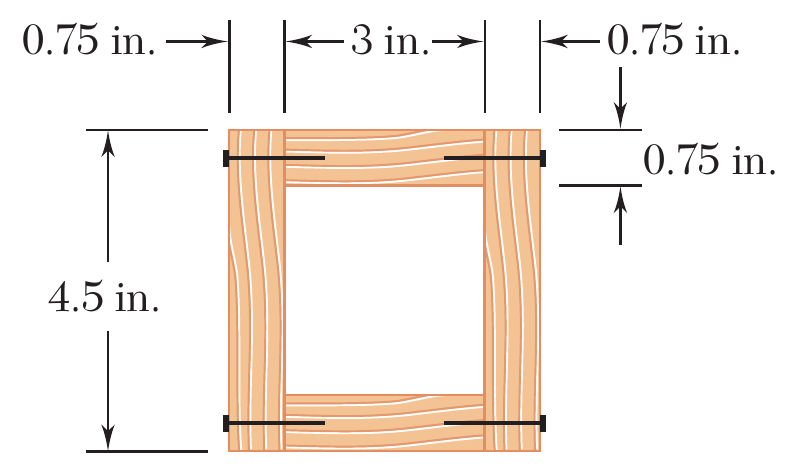
\includegraphics[width=\linewidth,height=5.5cm,keepaspectratio]{Chap_6/fig_6_25.png}
    \column{0.56\textwidth}
      \small
      Một dầm hộp vuông được ghép từ bốn tấm ván như hình vẽ. Biết khoảng
      cách giữa các đinh là 44 mm và dầm chịu lực cắt đứng có độ lớn
      $V = 2{,}5\,\mathrm{kN}$, xác định lực cắt trong mỗi đinh.

      \vspace{0.8em}
      \textbf{LỜI GIẢI:}
      \begin{itemize}
        \setlength{\itemsep}{0.5em}
        \item Xác định lực cắt trên một đơn vị chiều dài dọc theo mỗi mép của
              tấm ván trên.
        \item Dựa vào bước đinh, xác định lực cắt trong mỗi đinh.
      \end{itemize}
  \end{columns}
\end{frame}
% ===========
\begin{frame}[t]{Ví dụ 6.04 (tiếp)}
  \begin{columns}[T]
    \column{0.60\textwidth}
      \footnotesize
      \textbf{LỜI GIẢI:}
      \begin{itemize}
        \setlength{\itemsep}{0.20em}
        \item Xác định lực cắt trên một đơn vị chiều dài dọc theo mỗi mép của
              tấm ván trên.

              Với tấm ván trên:
        \[
          Q = A'\bar{y} = (18\,\mathrm{mm})(76\,\mathrm{mm})(47\,\mathrm{mm})
            = 64\,296\,\mathrm{mm}^3
        \]
              Với toàn bộ mặt cắt dầm:
        \[
          I = \tfrac{1}{12}(112\,\mathrm{mm})^4 - \tfrac{1}{12}(76\,\mathrm{mm})^4
            = 10{,}332\times10^{6}\,\mathrm{mm}^4
        \]
        \[
          q = \frac{VQ}{I} = \frac{(2500\,\mathrm{N})(64\,296\,\mathrm{mm}^3)}{10{,}332\times10^{6}\,\mathrm{mm}^4}
            = 15{,}6\,\mathrm{N/mm}
        \]
        \[
          f = \frac{q}{2} = 7{,}8\,\mathrm{N/mm}
        \]
        = lực trên một đơn vị chiều dài mỗi mép
        \item Dựa vào bước đinh, xác định lực cắt trong mỗi đinh:
        \[
          F = (44\,\mathrm{mm})f = (44\,\mathrm{mm})(7{,}8\,\mathrm{N/mm})
          \qquad \boxed{F = 343{,}2\,\mathrm{N}}
        \]
      \end{itemize}
    \column{0.38\textwidth}
      \centering
      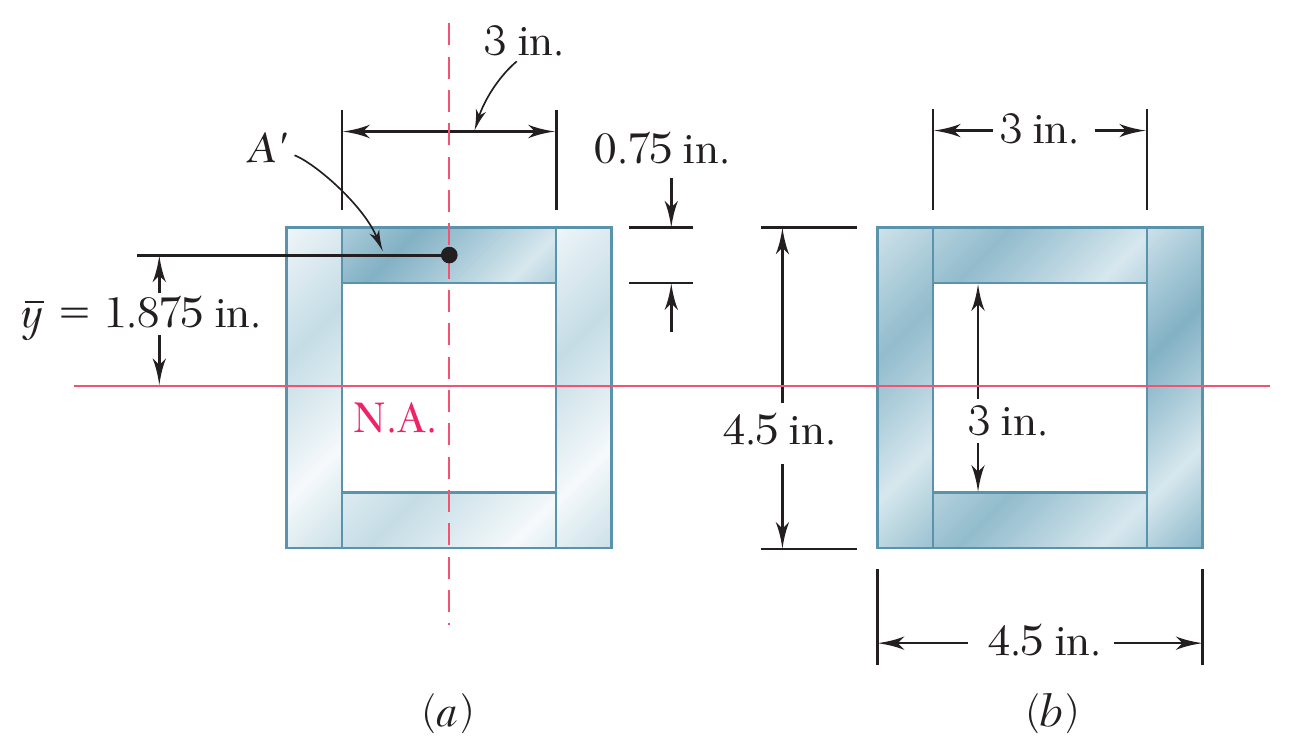
\includegraphics[width=\linewidth,height=4.7cm,keepaspectratio]{Chap_6/fig_6_26.png}
  \end{columns}
\end{frame}
% ===========
\section{Ứng suất tiếp trong cấu kiện thành mỏng}
\begin{frame}[t]{Ứng suất tiếp trong cấu kiện thành mỏng}
  \begin{columns}[T]
    \column{0.58\textwidth}
      \small
      \begin{itemize}
        \setlength{\itemsep}{0.5em}
        \item Xét một đoạn dầm cánh rộng chịu lực cắt đứng $V$.
        \item Lực cắt dọc trên phân tố là:
        \[
          \Delta H = \frac{VQ}{I}\Delta x
        \]
        \item Ứng suất tiếp tương ứng là:
        \[
          \tau_{zx} = \tau_{xz} \approx \frac{\Delta H}{t\Delta x} = \frac{VQ}{It}
        \]
        \item Trước đây đã nhận được biểu thức tương tự cho ứng suất tiếp
              trong bụng dầm:
        \[
          \tau_{xy} = \frac{VQ}{It}
        \]
        \item \textbf{LƯU Ý:} $\tau_{xy} \approx 0$ trong các cánh;
              $\tau_{xz} \approx 0$ trong bụng.
      \end{itemize}
    \column{0.40\textwidth}
      \centering
      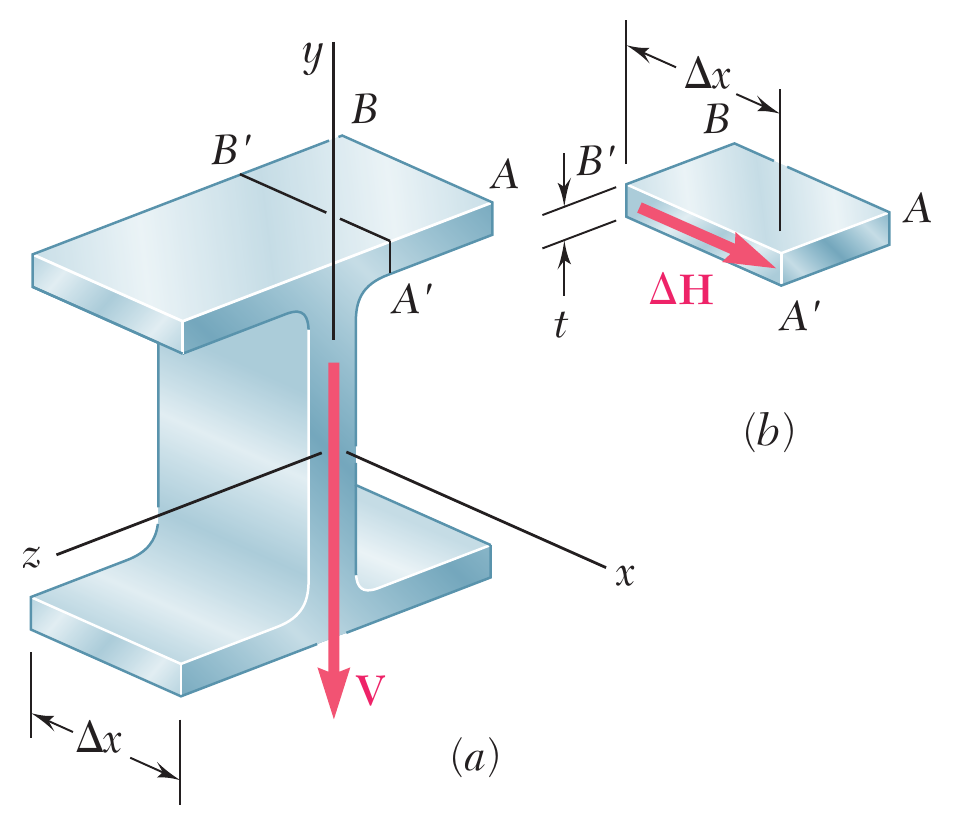
\includegraphics[width=\linewidth,height=2.9cm,keepaspectratio]{Chap_6/fig_6_27.png}\\[2pt]
      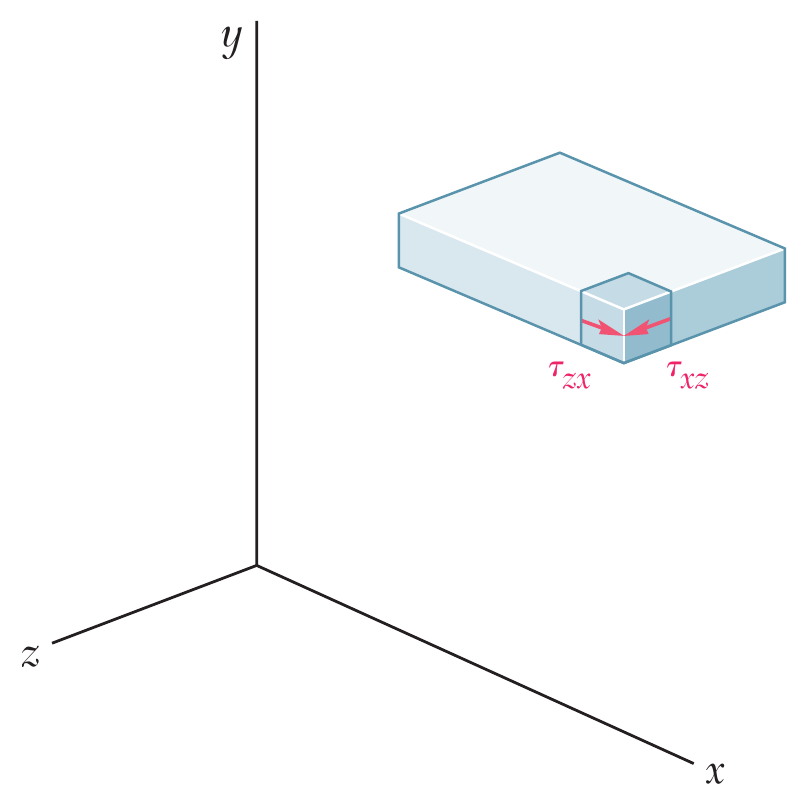
\includegraphics[width=\linewidth,height=2.9cm,keepaspectratio]{Chap_6/fig_6_28.png}
  \end{columns}
\end{frame}
% ===========
\begin{frame}[t]{Ứng suất tiếp trong cấu kiện thành mỏng (tiếp)}
  \begin{columns}[T]
    \column{0.58\textwidth}
      \small
      \begin{itemize}
        \setlength{\itemsep}{0.7em}
        \item Sự thay đổi dòng lực cắt trên mặt cắt chỉ phụ thuộc vào sự thay
              đổi của mô men tĩnh:
        \[
          q = \tau t = \frac{VQ}{I}
        \]
        \item Với dầm hộp, $q$ tăng liên tục từ không tại $A$ đến giá trị lớn
              nhất tại $C$ và $C'$, rồi giảm về không tại $E$.
        \item Chiều của $q$ trong các phần nằm ngang của mặt cắt có thể suy ra
              từ chiều trong các phần thẳng đứng hoặc từ chiều của lực cắt $V$.
      \end{itemize}
    \column{0.40\textwidth}
      \centering
      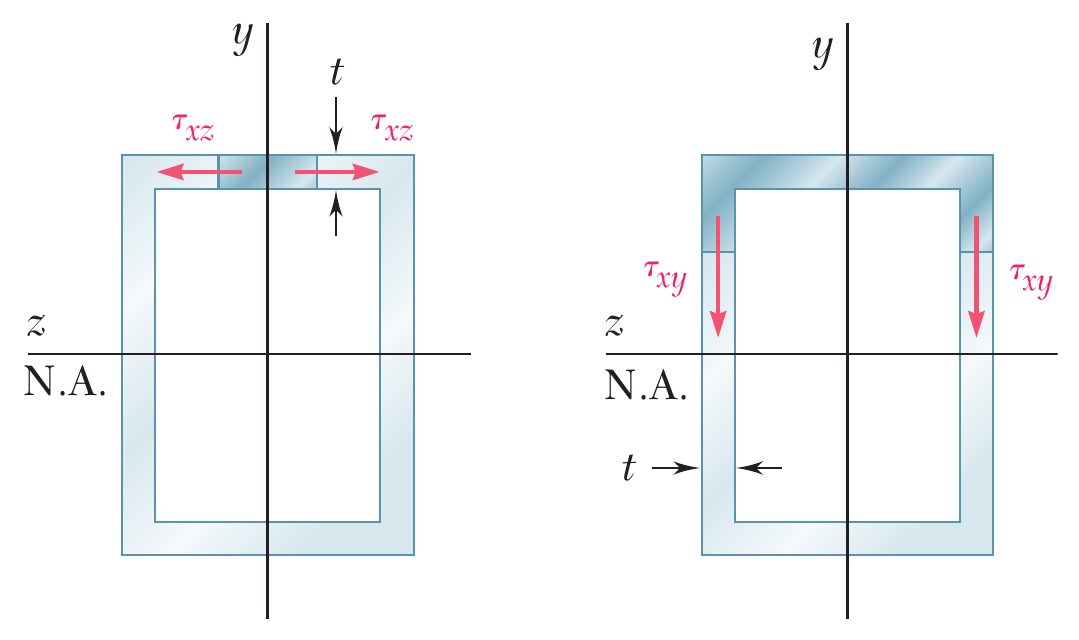
\includegraphics[width=\linewidth,height=2.9cm,keepaspectratio]{Chap_6/fig_6_30.png}\\[2pt]
      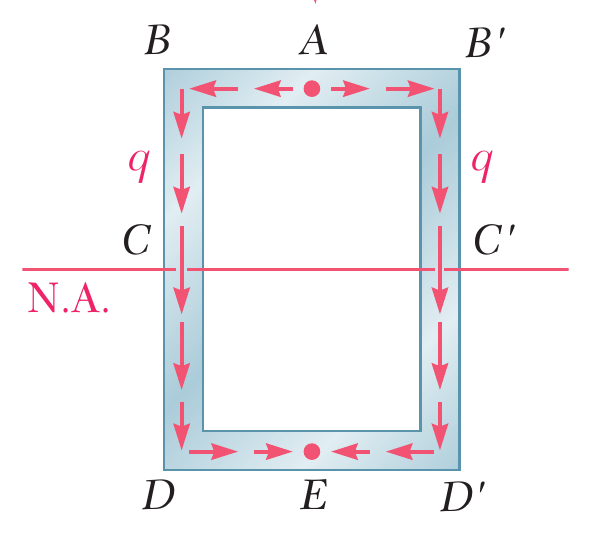
\includegraphics[width=\linewidth,height=2.9cm,keepaspectratio]{Chap_6/fig_6_32.png}
  \end{columns}
\end{frame}
% ===========
\begin{frame}[t]{Ứng suất tiếp trong cấu kiện thành mỏng (tiếp)}
  \begin{columns}[T]
    \column{0.58\textwidth}
      \small
      \begin{itemize}
        \setlength{\itemsep}{0.9em}
        \item Với dầm cánh rộng, dòng lực cắt tăng đối xứng từ không tại $A$
              và $A'$, đạt cực đại tại $C$ rồi giảm về không tại $E$ và $E'$.
        \item Tính liên tục của sự biến thiên $q$ và sự hợp dòng $q$ từ các
              nhánh của mặt cắt gợi ý sự tương tự với dòng chảy chất lỏng.
      \end{itemize}
    \column{0.40\textwidth}
      \centering
      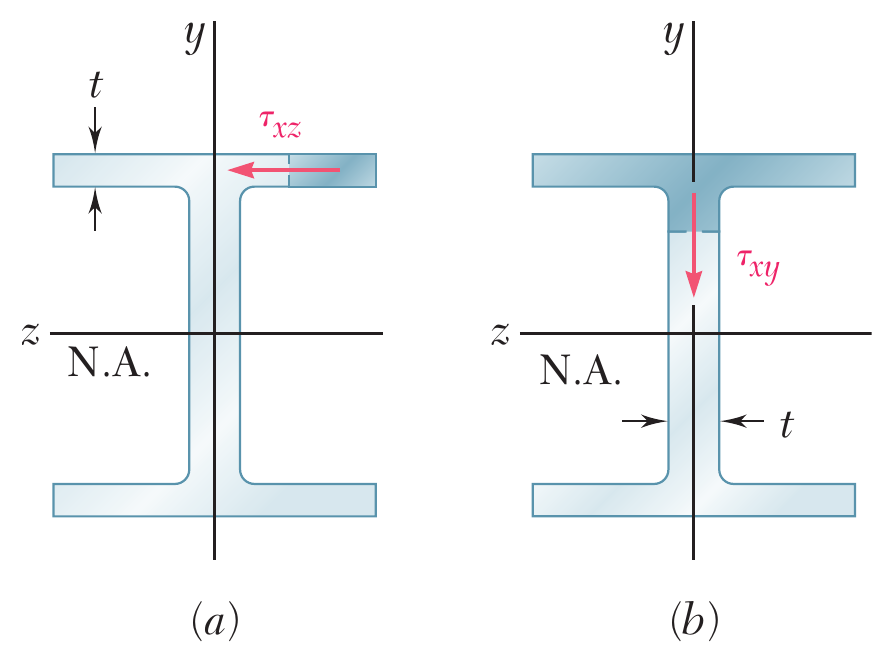
\includegraphics[width=\linewidth,height=2.9cm,keepaspectratio]{Chap_6/fig_6_29.png}\\[2pt]
      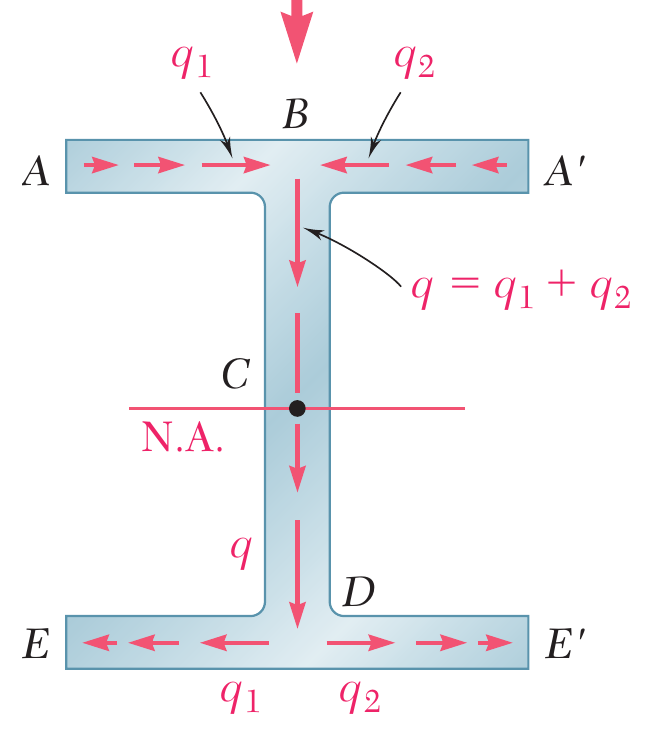
\includegraphics[width=\linewidth,height=2.9cm,keepaspectratio]{Chap_6/fig_6_33.png}
  \end{columns}
\end{frame}
% ===========
\section{Biến dạng dẻo}
\begin{frame}[t]{Biến dạng dẻo}
  \begin{columns}[T]
    \column{0.58\textwidth}
      \footnotesize
      \begin{itemize}
        \setlength{\itemsep}{0.20em}
        \item Nhắc lại:
              $\displaystyle M_Y = \frac{I}{c}\sigma_Y$ = mô men đàn hồi lớn nhất
        \item Với $M = PL < M_Y$, ứng suất pháp không vượt quá giới hạn chảy
              tại bất kỳ điểm nào dọc theo dầm.
        \item Với $PL > M_Y$, chảy dẻo bắt đầu tại $B$ và $B'$. Với vật liệu
              đàn -- dẻo, nửa chiều dày lõi đàn hồi được xác định từ:
        \[
          Px = \tfrac{3}{2}M_Y\left(1 - \tfrac{1}{3}\frac{y_Y^2}{c^2}\right)
        \]
        \item Mặt cắt tại ngàm trở nên dẻo hoàn toàn ($y_Y = 0$) khi:
        \[
          PL = \tfrac{3}{2}M_Y = M_p
        \]
        \item Tải trọng lớn nhất mà dầm có thể chịu được:
        \[
          P_{\max} = \frac{M_p}{L}
        \]
      \end{itemize}
    \column{0.40\textwidth}
      \centering
      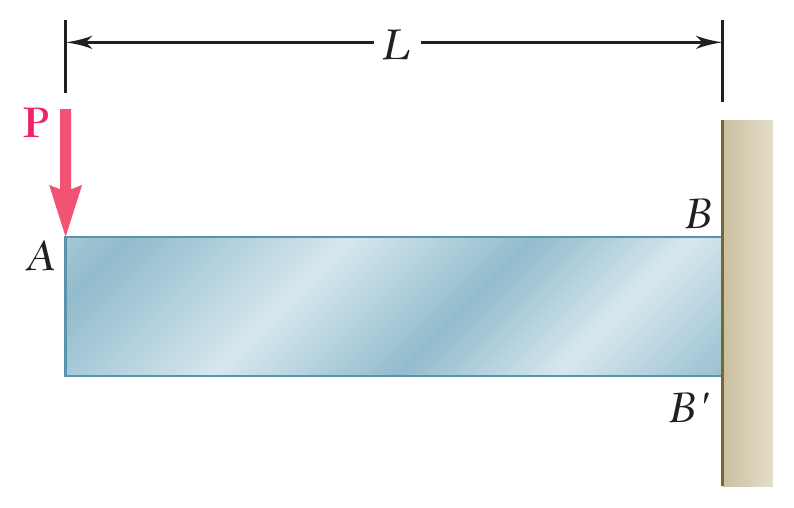
\includegraphics[width=\linewidth,height=1.6cm,keepaspectratio]{Chap_6/fig_6_34.png}\\[2pt]
      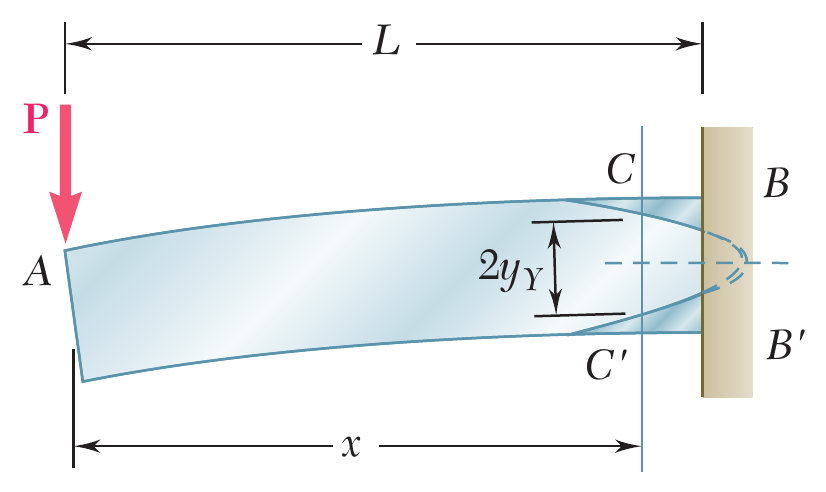
\includegraphics[width=\linewidth,height=1.6cm,keepaspectratio]{Chap_6/fig_6_35.png}\\[2pt]
      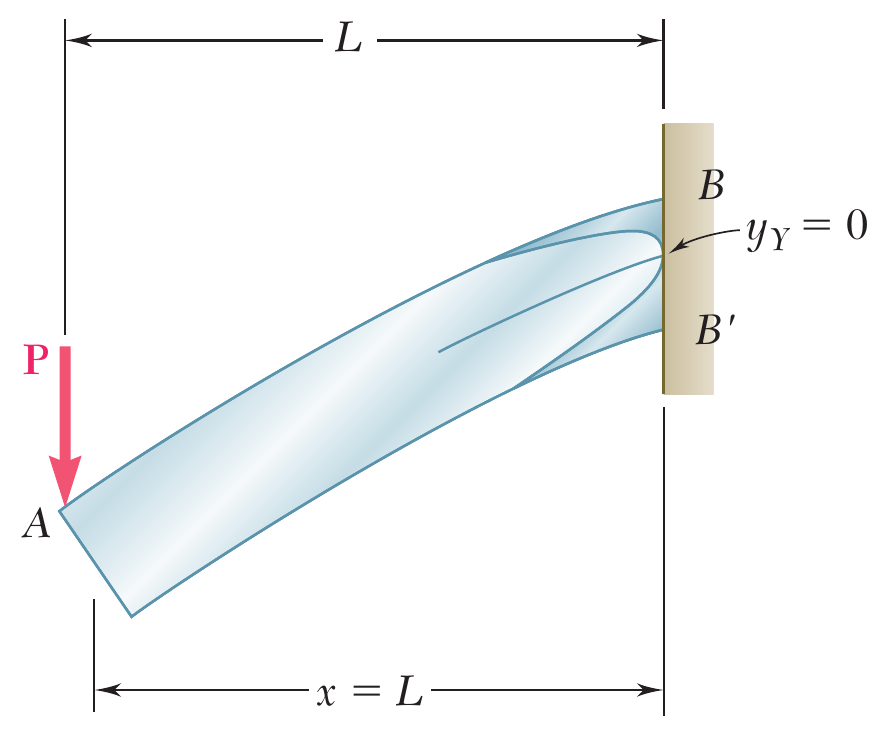
\includegraphics[width=\linewidth,height=1.6cm,keepaspectratio]{Chap_6/fig_6_36.png}
  \end{columns}
\end{frame}
% ===========
\begin{frame}[t]{Biến dạng dẻo (tiếp)}
  \begin{columns}[T]
    \column{0.58\textwidth}
      \small
      \begin{itemize}
        \setlength{\itemsep}{0.4em}
        \item Phần thảo luận trên chỉ dựa trên ứng suất pháp.
        \item Xét lực cắt ngang trên một phân tố nằm trong vùng dẻo:
        \[
          \Delta H = -\int(\sigma_C - \sigma_D)\,dA
            = -\int(\sigma_Y - \sigma_Y)\,dA = 0
        \]
        Do đó ứng suất tiếp bằng không trong vùng dẻo.
        \item Lực cắt do lõi đàn hồi chịu:
        \[
          \tau_{xy} = \frac{3}{2}\frac{P}{A'}\left(1 - \frac{y^2}{y_Y^2}\right)
          \qquad A' = 2by_Y
        \]
        \[
          \tau_{\max} = \frac{3}{2}\frac{P}{A'}
        \]
        \item Khi $A'$ giảm, $\tau_{\max}$ tăng và có thể vượt quá $\tau_Y$.
      \end{itemize}
    \column{0.40\textwidth}
      \centering
      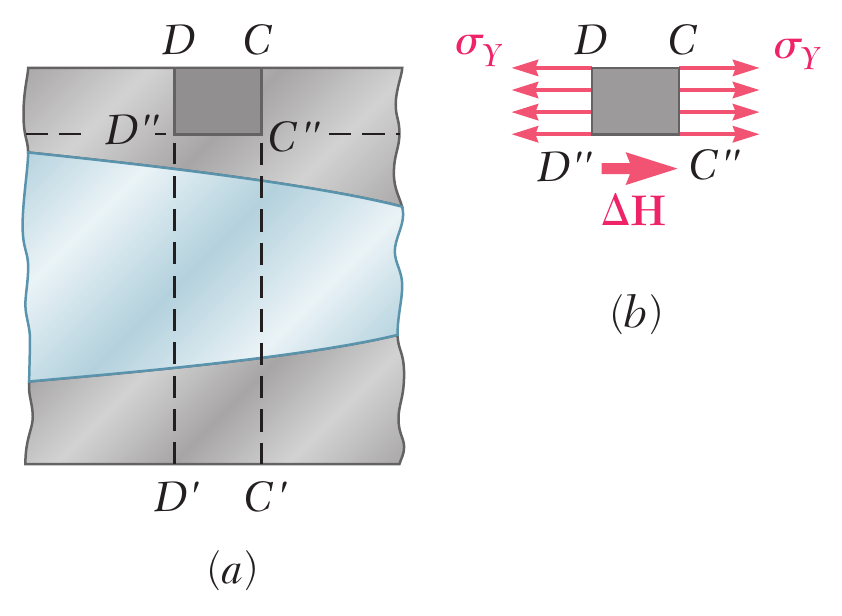
\includegraphics[width=\linewidth,height=2.9cm,keepaspectratio]{Chap_6/fig_6_37.png}\\[2pt]
      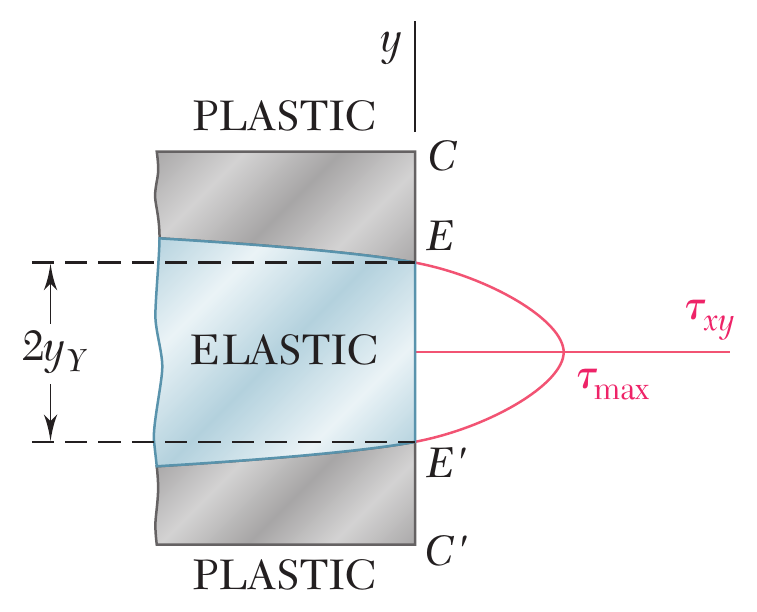
\includegraphics[width=\linewidth,height=2.9cm,keepaspectratio]{Chap_6/fig_6_38.png}
  \end{columns}
\end{frame}
% ===========
\section{Bài mẫu 6.3}
\begin{frame}[t]{Bài mẫu 6.3}
  \begin{columns}[T]
    \column{0.42\textwidth}
      \centering
      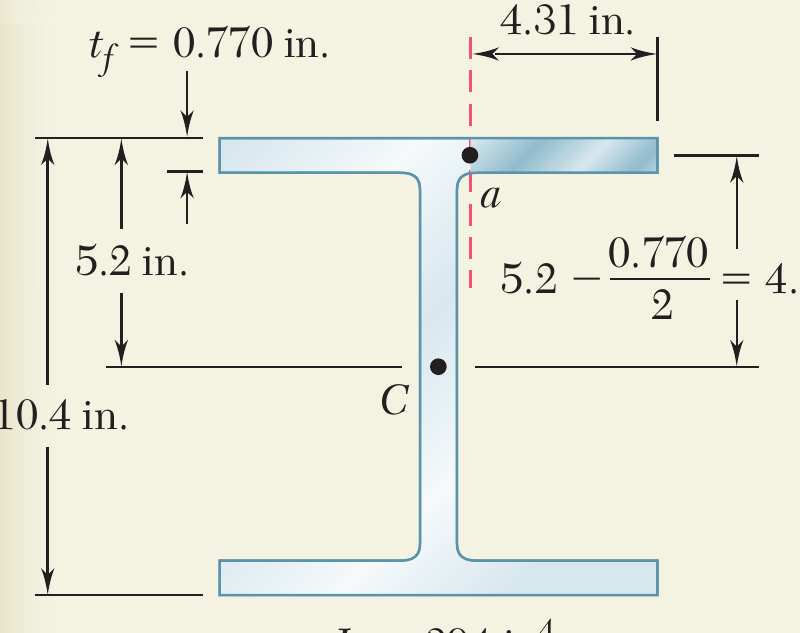
\includegraphics[width=\linewidth,height=5.5cm,keepaspectratio]{Chap_6/sp_6_3.png}
    \column{0.56\textwidth}
      \small
      Biết lực cắt đứng là 200 kN trong dầm thép cán W250$\times$101, xác
      định ứng suất tiếp nằm ngang trong cánh trên tại điểm $a$.

      \vspace{0.8em}
      \textbf{LỜI GIẢI:}
      \begin{itemize}
        \setlength{\itemsep}{0.5em}
        \item Với phần diện tích được tô đậm:
        \[
          Q = (108\,\mathrm{mm})(19{,}6\,\mathrm{mm})(122{,}2\,\mathrm{mm})
            = 258\,700\,\mathrm{mm}^3
        \]
        \item Ứng suất tiếp tại $a$:
        \[
          \tau = \frac{VQ}{It}
            = \frac{(200\times10^{3}\,\mathrm{N})(258{,}7\times10^{-6}\,\mathrm{m}^3)}
                   {(164\times10^{-6}\,\mathrm{m}^4)(0{,}0196\,\mathrm{m})}
        \]
        \[
          \boxed{\tau = 16{,}1\,\mathrm{MPa}}
        \]
      \end{itemize}
  \end{columns}
\end{frame}
% ===========
\section{Tải trọng không đối xứng trên cấu kiện thành mỏng}
\begin{frame}[t]{Tải trọng không đối xứng trên cấu kiện thành mỏng}
  \begin{columns}[T]
    \column{0.49\textwidth}
      \small
      \begin{itemize}
        \item Dầm chịu tải trong mặt phẳng đối xứng thẳng đứng biến dạng
              trong mặt phẳng đối xứng mà không bị xoắn:
      \end{itemize}
      \[
        \sigma_x = -\frac{My}{I} \qquad \tau_{\mathrm{tb}} = \frac{VQ}{It}
      \]
      \centering
      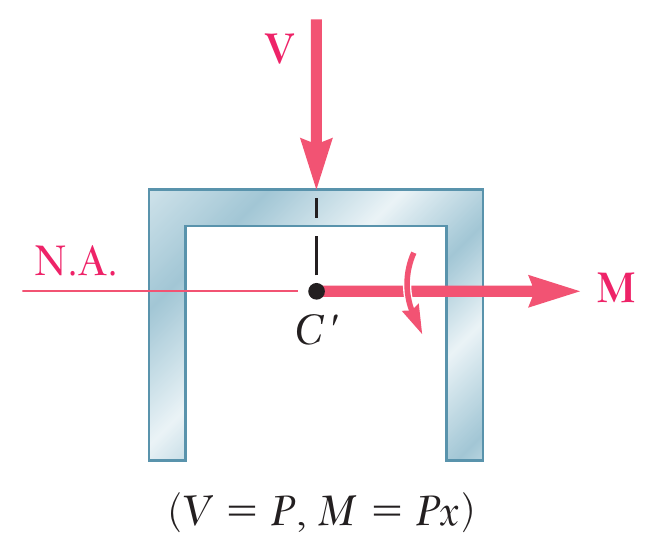
\includegraphics[width=0.49\linewidth,height=2.9cm,keepaspectratio]{Chap_6/fig_6_40.png}\hfill
      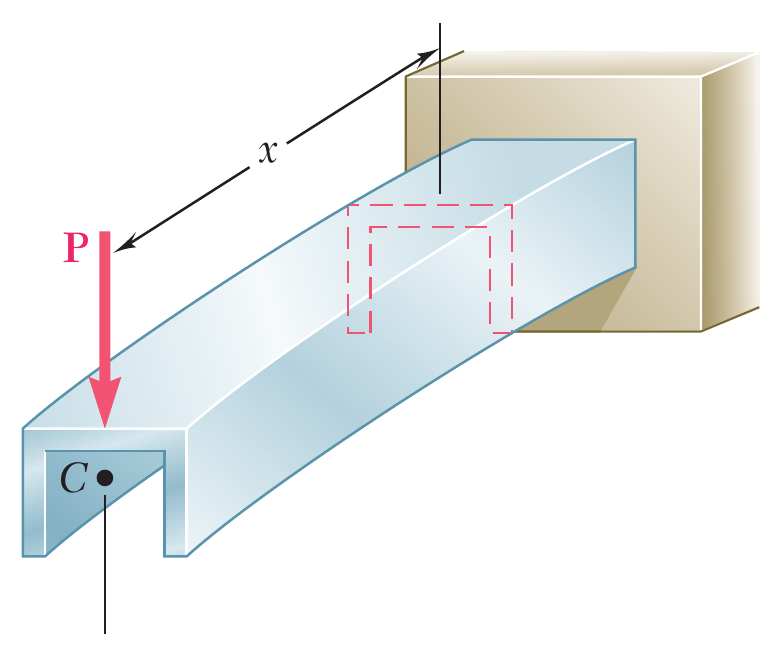
\includegraphics[width=0.49\linewidth,height=2.9cm,keepaspectratio]{Chap_6/fig_6_39.png}
    \column{0.49\textwidth}
      \small
      \begin{itemize}
        \item Dầm không có mặt phẳng đối xứng thẳng đứng bị uốn và xoắn khi
              chịu tải:
      \end{itemize}
      \[
        \sigma_x = -\frac{My}{I} \qquad \tau_{\mathrm{tb}} \neq \frac{VQ}{It}
      \]
      \centering
      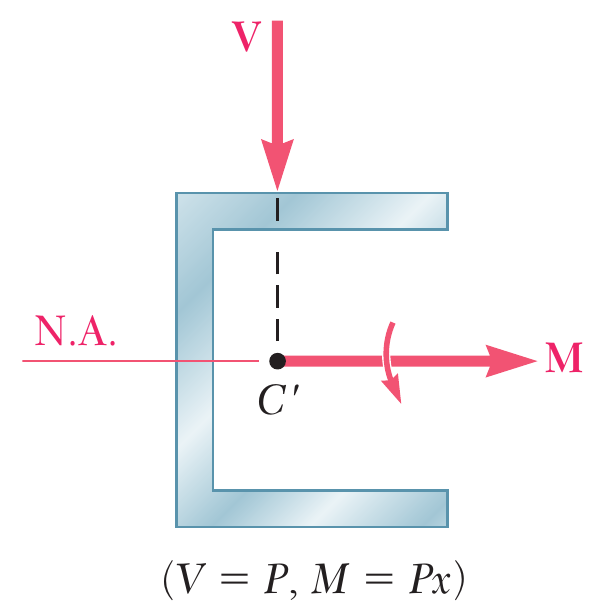
\includegraphics[width=0.49\linewidth,height=2.9cm,keepaspectratio]{Chap_6/fig_6_41.png}\hfill
      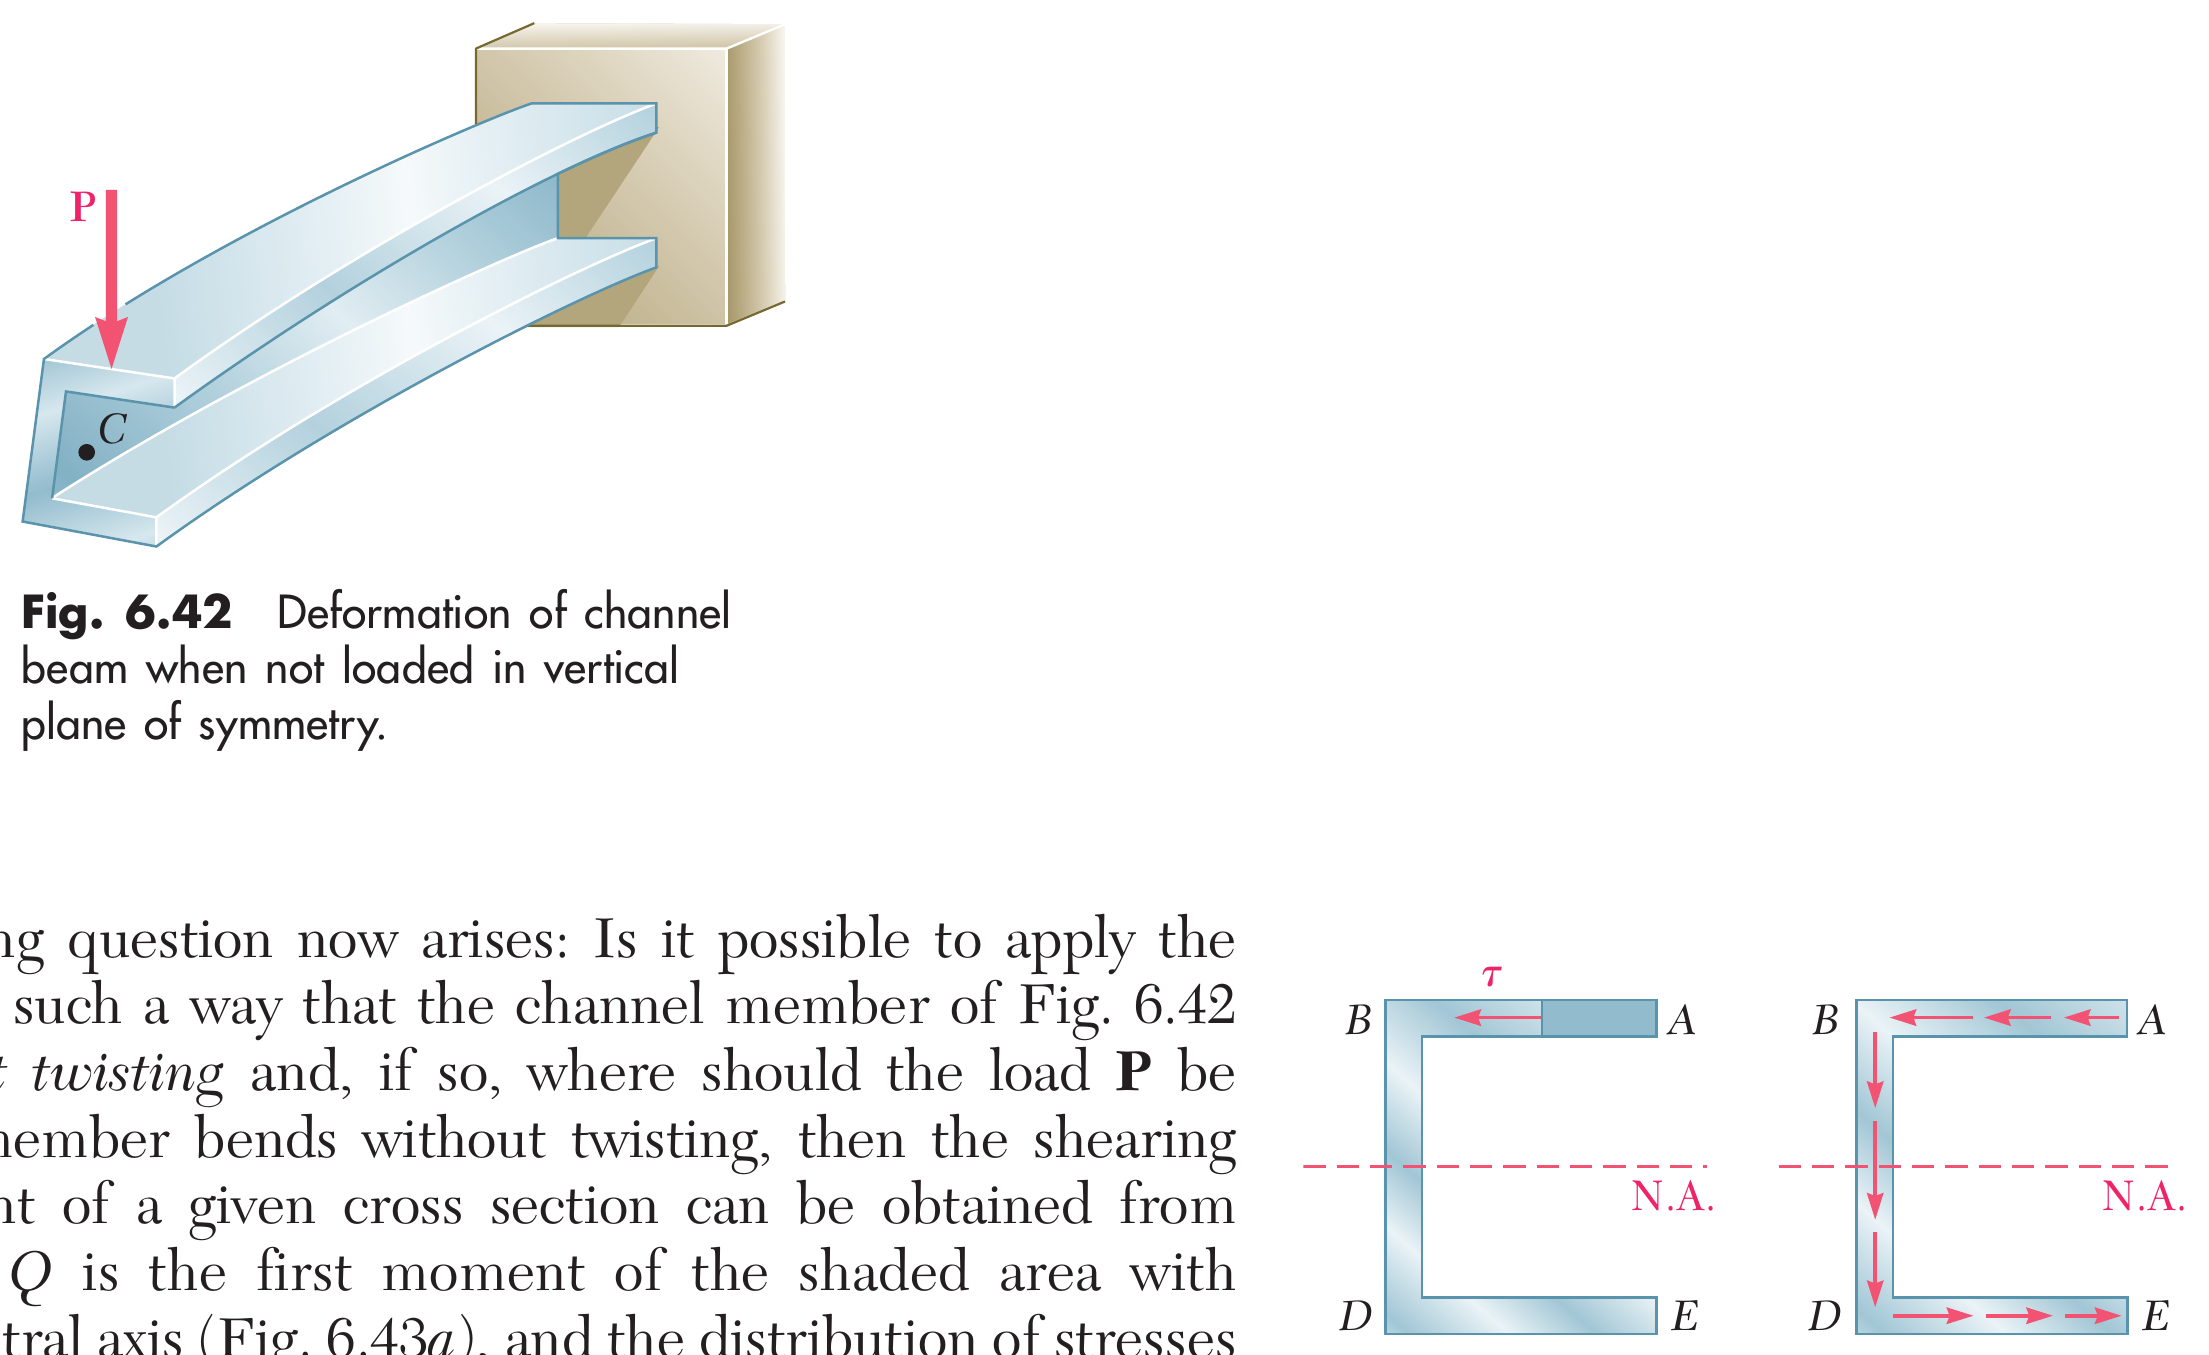
\includegraphics[width=0.49\linewidth,height=2.9cm,keepaspectratio]{Chap_6/fig_6_42.png}
  \end{columns}
\end{frame}
% ===========
\begin{frame}[t]{Tải trọng không đối xứng trên cấu kiện thành mỏng (tiếp)}
  \begin{columns}[T]
    \column{0.58\textwidth}
      \footnotesize
      \begin{itemize}
        \setlength{\itemsep}{0.20em}
        \item Nếu lực cắt được đặt sao cho dầm không bị xoắn, phân bố ứng
              suất tiếp thỏa mãn:
        \[
          \tau_{\mathrm{tb}} = \frac{VQ}{It} \qquad
          V = \int_B^D q\,ds
        \]
        \[
          F = \int_A^B q\,ds = -\int_D^E q\,ds = -F'
        \]
        \item $F$ và $F'$ tạo thành một ngẫu lực $Fh$, cho thấy cần đặt thêm
              một mô men xoắn bên cạnh lực cắt:
        \[
          Fh = Ve
        \]
        \item Khi lực $P$ đặt cách đường tâm bụng một khoảng $e$ về bên trái,
              cấu kiện bị uốn trong mặt phẳng thẳng đứng mà không bị xoắn.
        \item Điểm $O$ được gọi là \emph{tâm uốn} (tâm cắt) của mặt cắt dầm.
      \end{itemize}
    \column{0.40\textwidth}
      \centering
      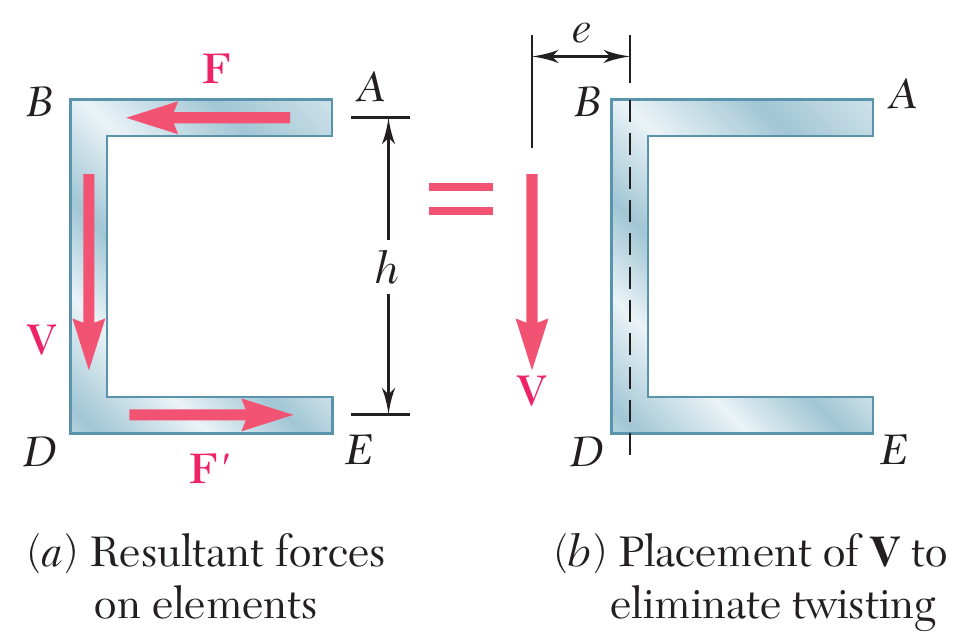
\includegraphics[width=\linewidth,height=2.5cm,keepaspectratio]{Chap_6/fig_6_45.png}\\[2pt]
      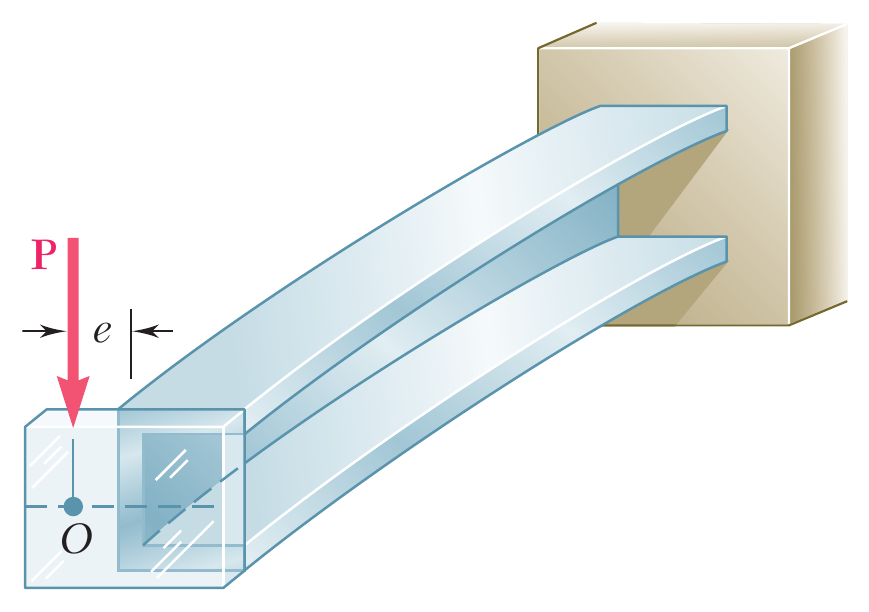
\includegraphics[width=\linewidth,height=2.5cm,keepaspectratio]{Chap_6/fig_6_46.png}
  \end{columns}
\end{frame}
% ===========
\section{Ví dụ 6.05}
\begin{frame}[t]{Ví dụ 6.05}
  \begin{columns}[T]
    \column{0.60\textwidth}
      \small
      \begin{itemize}
        \setlength{\itemsep}{0.4em}
        \item Xác định vị trí tâm uốn của mặt cắt chữ C (thép chữ U) với
              $b = 100\,\mathrm{mm}$, $h = 150\,\mathrm{mm}$ và
              $t = 4\,\mathrm{mm}$:
        \[
          e = \frac{Fh}{V}
        \]
        \[
          F = \int_0^b q\,ds = \int_0^b\frac{VQ}{I}\,ds
            = \frac{V}{I}\int_0^b st\frac{h}{2}\,ds = \frac{Vthb^2}{4I}
        \]
        \[
          I = I_{\text{bụng}} + 2I_{\text{cánh}}
            = \tfrac{1}{12}th^3 + 2\left[\tfrac{1}{12}bt^3 + bt\left(\tfrac{h}{2}\right)^2\right]
        \]
        \[
          I \cong \tfrac{1}{12}th^2(6b + h)
        \]
        \item Kết hợp lại:
        \[
          e = \frac{b}{2 + \dfrac{h}{3b}}
            = \frac{100\,\mathrm{mm}}{2 + \dfrac{150\,\mathrm{mm}}{3(100\,\mathrm{mm})}}
          \qquad \boxed{e = 40\,\mathrm{mm}}
        \]
      \end{itemize}
    \column{0.38\textwidth}
      \centering
      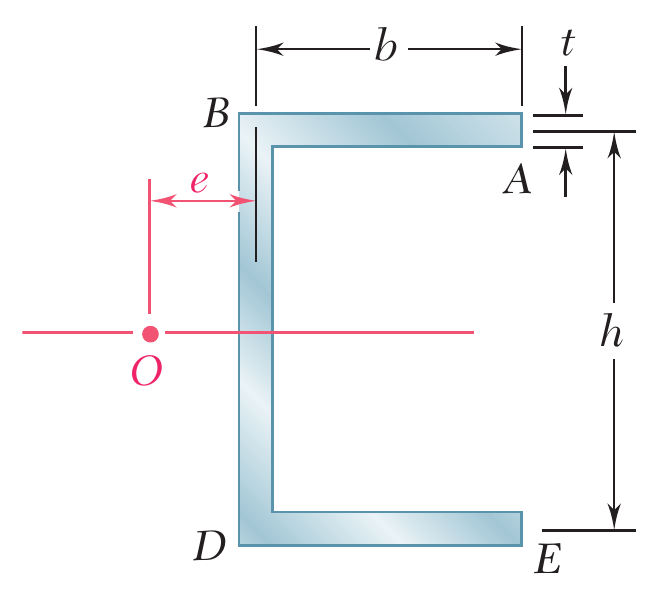
\includegraphics[width=\linewidth,height=2.9cm,keepaspectratio]{Chap_6/fig_6_48.png}\\[2pt]
      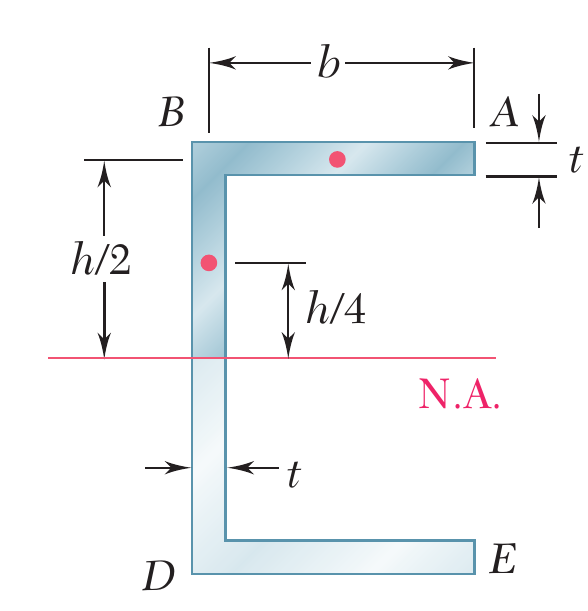
\includegraphics[width=\linewidth,height=2.9cm,keepaspectratio]{Chap_6/ex_6_06.png}
  \end{columns}
\end{frame}
% ===========
\section{Ví dụ 6.06}
\begin{frame}[t]{Ví dụ 6.06}
  \begin{columns}[T]
    \column{0.62\textwidth}
      \scriptsize
      \begin{itemize}
        \setlength{\itemsep}{0.20em}
        \item Xác định phân bố ứng suất tiếp với $V = 10\,\mathrm{kN}$:
        \[
          \tau = \frac{q}{t} = \frac{VQ}{It}
        \]
        \item Ứng suất tiếp trong các cánh:
        \[
          \tau = \frac{VQ}{It} = \frac{V}{It}\,st\frac{h}{2} = \frac{Vh}{2I}s
        \]
        \[
          \tau_B = \frac{Vhb}{2\left[\frac{1}{12}th^2(6b + h)\right]}
            = \frac{6Vb}{th(6b + h)}
        \]
        \[
          \tau_B = \frac{6(10\,000\,\mathrm{N})(0{,}1\,\mathrm{m})}
                        {(0{,}004\,\mathrm{m})(0{,}15\,\mathrm{m})(6\times0{,}1 + 0{,}15)\,\mathrm{m}}
            = 13{,}3\,\mathrm{MPa}
        \]
        \item Ứng suất tiếp trong bụng:
        \[
          \tau_{\max} = \frac{VQ}{It}
            = \frac{V\left[\frac{1}{8}ht(4b + h)\right]}{\frac{1}{12}th^2(6b + h)\,t}
            = \frac{3V(4b + h)}{2th(6b + h)}
        \]
        \[
          \tau_{\max} = \frac{3(10\,000\,\mathrm{N})(4\times0{,}1 + 0{,}15)\,\mathrm{m}}
                             {2(0{,}004\,\mathrm{m})(0{,}15\,\mathrm{m})(6\times0{,}1 + 0{,}15)\,\mathrm{m}}
            = 18{,}3\,\mathrm{MPa}
        \]
      \end{itemize}
    \column{0.36\textwidth}
      \centering
      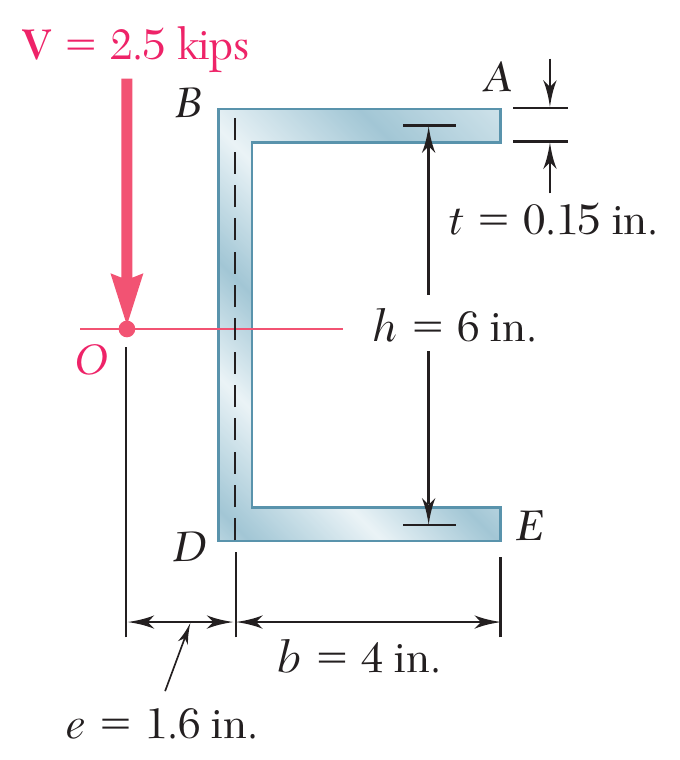
\includegraphics[width=\linewidth,height=4.7cm,keepaspectratio]{Chap_6/fig_6_50.png}
  \end{columns}
\end{frame}

\end{document}
